\documentclass[11pt]{article}

\usepackage[review]{acl}
\usepackage{times}
\usepackage{latexsym}
\usepackage[T1]{fontenc}
\usepackage[utf8]{inputenc}
\usepackage{microtype}
\usepackage{xspace}
\usepackage{amsmath,amssymb,amsthm}
\usepackage{booktabs}
\usepackage{placeins}
\usepackage{graphicx}
\usepackage{algorithm}
\usepackage{algpseudocode}
\usepackage{tikz}
\usetikzlibrary{arrows.meta,positioning,calc,shapes.geometric}

\definecolor{fsblue}{HTML}{1F4E79}
\definecolor{fsorange}{HTML}{C45911}
\definecolor{fsgreen}{HTML}{1B7A3A}
\definecolor{fspurple}{HTML}{5B2C6F}
\definecolor{fsgray}{HTML}{5D6D7E}
\definecolor{fslight}{HTML}{E8F1F8}
\definecolor{fsspec}{HTML}{FDEBD0}
\definecolor{fscommit}{HTML}{E5F6EA}
\definecolor{fsmiss}{HTML}{F8E8E8}
\definecolor{fsred}{HTML}{B00020}
\definecolor{fsgain}{HTML}{0B6E4F}

\newcommand{\sys}{\mbox{\textsc{PD-Prune}}\xspace}
\newtheorem{proposition}{Proposition}
\newtheorem*{proposition*}{Proposition}

\title{\sys{}: Split Prefill and Decode Pruning\\ for Efficient Agentic Inference}

\author{Anonymous ACL submission}

\begin{document}
\maketitle

\begin{abstract}
Large language models used as agents expand one committed trunk into several residuals and later keep a single spine.
This serving pattern is inefficient: search and early-stop methods score tokens that have already been generated, so residuals that will be aborted still pay GPU prefill, KV transfer, and decode until a prune score exists.
The waste stems from the stack's inability to refuse a residual before tokens or pages exist.
We propose \sys, which reduces that waste by identifying and pruning abortable residuals during KV-cache encoding of the residual, then deciding continuation from a short generated prefix.
The pruning steers the stack toward treating a loop as skippable text rather than as a thought to encode, while a separate decode score preserves residuals that can still solve once a prefix is visible.
To identify what to prune, we introduce two unshared scores with ordered bars $(\tau_{\mathrm{pre}}, \tau_{\mathrm{dec}})$, and we connect the prefill bar to an invariance of prefill work across decode-time hosts.
Our approach does not replace the host's cut or incur extra model calls at test time.
Experiments show that \sys reduces the prefill shared by three decode-time pruners while preserving any-finished accuracy, and that a short probe restores full MATH-500 accuracy at lower end-to-end time.
\end{abstract}

\section{Introduction}
\label{sec:intro}

The rapid adoption of large language models as agents~\citep{tot,react,selfconsistency} has turned inference from a single continuation into a search process.
An agentic step expands a committed trunk of length $L$ into $k$ residuals and later keeps a single spine (Figure~\ref{fig:problem}).
This pattern is the serving unit of Tree-of-Thoughts, self-consistency, and tool-using loops, and it is where latency and memory are spent.
However, existing stacks exhibit a critical inefficiency: residuals that the search will abort still incur GPU prefill, KV transfer, and decode until a prune score exists.
That waste grows with fan-out width and is paid on every step, posing a significant cost to the reliability of agentic inference in real-world applications.

The susceptibility of LLM serving to this waste stems from a fundamental limitation in parsing the fan-out, i.e., the inability to distinguish a residual that must be encoded from one that can be refused as text~\citep{esc,specrej,dpts}.
In reducing that cost, replacing the search algorithm, or retraining the model to emit fewer thoughts, can be computationally prohibitive and is orthogonal to serving.
Alternatively, existing mitigation strategies focus on scoring tokens that have already been generated~\citep{esc,specrej,dpts}, on recording a prefix only after a full block is hashed~\citep{vllm,sglang}, or on transferring every page a disaggregated prefiller has computed~\citep{distserve,splitwise}.
Such strategies often provide only decode-side savings, or they ship KV that the search is about to drop.
Additionally, imposing a single threshold on both prefill and decode can drop residuals that still solve, thereby undermining the quality of the kept spine.

\begin{figure*}[t]
\centering
\resizebox{\textwidth}{!}{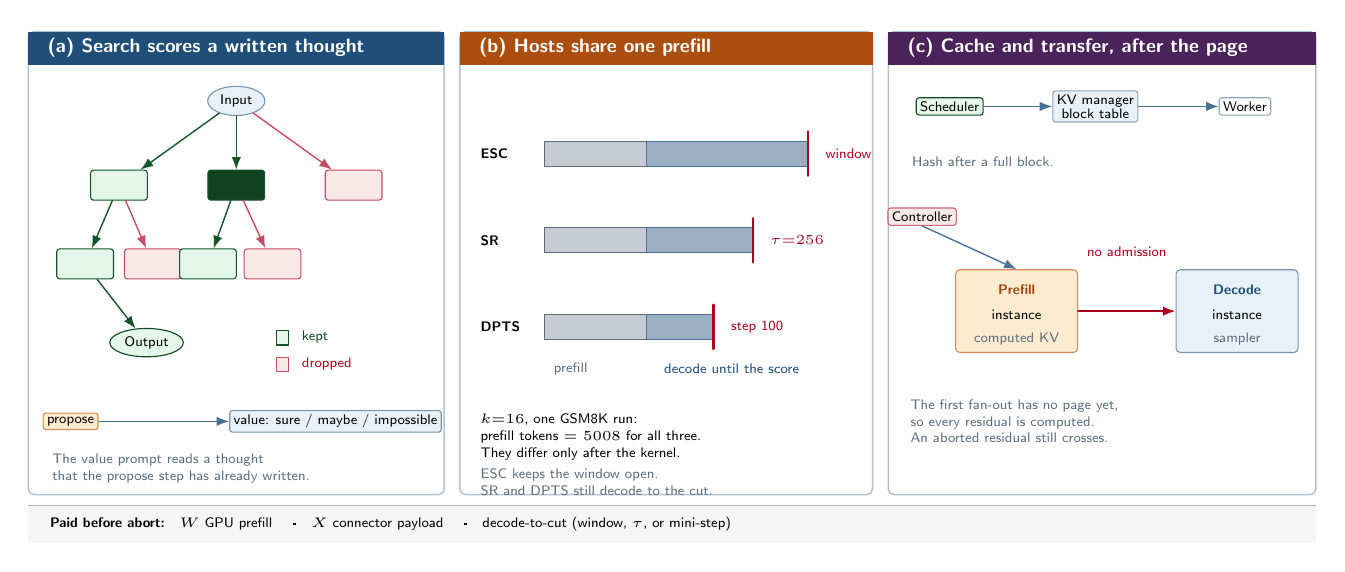
\begin{tikzpicture}[
  x=1cm, y=1cm,
  font=\sffamily\scriptsize,
  >=Latex,
  line cap=round, line join=round,
  panel/.style={draw=fsblue!35, line width=0.55pt, rounded corners=2pt, fill=white},
  head/.style={font=\scriptsize\bfseries\sffamily, text=white, anchor=west},
  chip/.style={draw, rounded corners=1pt, inner sep=1.4pt, font=\tiny\sffamily, line width=0.4pt},
  arr/.style={-{Latex[length=1.6mm,width=1.2mm]}, line width=0.5pt, draw=fsblue!80},
  thought/.style={draw, rounded corners=1pt, minimum width=0.72cm, minimum height=0.38cm, inner sep=0pt, font=\tiny\sffamily},
]
\path (0,0) rectangle (16.35,6.55);

% ---------- panels ----------
\draw[panel] (0.00,0.62) rectangle (5.28,6.50);
\draw[panel] (5.48,0.62) rectangle (10.72,6.50);
\draw[panel] (10.92,0.62) rectangle (16.35,6.50);
\fill[fsblue] (0.00,6.08) rectangle (5.28,6.50);
\fill[fsorange!88!black] (5.48,6.08) rectangle (10.72,6.50);
\fill[fspurple!80!black] (10.92,6.08) rectangle (16.35,6.50);
\node[head] at (0.12,6.29) {(a) Search scores a written thought};
\node[head] at (5.60,6.29) {(b) Hosts share one prefill};
\node[head] at (11.04,6.29) {(c) Cache and transfer, after the page};

% ---------- (a) ToT-style tree, original redraw ----------
\node[draw=fsblue!60, fill=fslight, ellipse, inner sep=1.5pt, font=\tiny\sffamily] (inp) at (2.64,5.62) {Input};
\node[thought, fill=fscommit, draw=fsgreen!70!black] (t0) at (1.15,4.55) {};
\node[thought, fill=fsgreen!55!black, draw=fsgreen!70!black] (t1) at (2.64,4.55) {};
\node[thought, fill=fsmiss, draw=fsred!70] (t2) at (4.13,4.55) {};
\node[thought, fill=fscommit, draw=fsgreen!70!black] (t00) at (0.72,3.55) {};
\node[thought, fill=fsmiss, draw=fsred!70] (t01) at (1.58,3.55) {};
\node[thought, fill=fscommit, draw=fsgreen!70!black] (t10) at (2.28,3.55) {};
\node[thought, fill=fsmiss, draw=fsred!70] (t11) at (3.10,3.55) {};
\node[draw=fsgreen!60!black, fill=fscommit, ellipse, inner sep=1.4pt, font=\tiny\sffamily] (out) at (1.50,2.55) {Output};
\draw[arr, draw=fsgreen!70!black] (inp) -- (t0);
\draw[arr, draw=fsgreen!70!black] (inp) -- (t1);
\draw[arr, draw=fsred!70] (inp) -- (t2);
\draw[arr, draw=fsgreen!70!black] (t0) -- (t00);
\draw[arr, draw=fsred!70] (t0) -- (t01);
\draw[arr, draw=fsgreen!70!black] (t1) -- (t10);
\draw[arr, draw=fsred!70] (t1) -- (t11);
\draw[arr, draw=fsgreen!70!black] (t00) -- (out);
\node[font=\tiny\sffamily, text=fsgreen!60!black, anchor=west] at (3.35,2.62) {kept};
\node[font=\tiny\sffamily, text=fsred, anchor=west] at (3.35,2.28) {dropped};
\fill[fscommit] (3.15,2.52) rectangle (3.30,2.70);
\draw[fsgreen!70!black] (3.15,2.52) rectangle (3.30,2.70);
\fill[fsmiss] (3.15,2.18) rectangle (3.30,2.36);
\draw[fsred!70] (3.15,2.18) rectangle (3.30,2.36);

\node[chip, draw=fsorange!70, fill=fsspec, anchor=west] (prop) at (0.18,1.55) {propose};
\node[chip, draw=fsblue!60, fill=fslight, anchor=west] (val) at (2.55,1.55) {value: sure / maybe / impossible};
\draw[arr] (prop.east) -- (val.west);
\node[font=\tiny\sffamily, text=fsgray, align=left, anchor=west] at (0.18,0.95)
  {The value prompt reads a thought\\that the propose step has already written.};

% ---------- (b) three hosts, identical prefill ----------
\foreach \y/\name/\dw/\cut in {
  4.95/ESC/2.05/window,
  3.85/SR/1.35/{$\tau{=}256$},
  2.75/DPTS/0.85/{step 100}
} {
  \node[font=\tiny\sffamily\bfseries, anchor=west] at (5.62,\y) {\name};
  \fill[fsgray!35] (6.55,\y-0.16) rectangle (7.85,\y+0.16);
  \draw[fsgray] (6.55,\y-0.16) rectangle (7.85,\y+0.16);
  \fill[fsblue!45] (7.85,\y-0.16) rectangle ({7.85+\dw},\y+0.16);
  \draw[fsblue!80] (7.85,\y-0.16) rectangle ({7.85+\dw},\y+0.16);
  \draw[fsred, line width=0.9pt] ({7.85+\dw},\y-0.28) -- ({7.85+\dw},\y+0.28);
  \node[font=\tiny\sffamily, text=fsred, anchor=west] at ({7.95+\dw},\y) {\cut};
}
\node[font=\tiny\sffamily, text=fsgray, anchor=west] at (6.55,2.22) {prefill};
\node[font=\tiny\sffamily, text=fsblue, anchor=west] at (7.95,2.22) {decode until the score};
\node[font=\tiny\sffamily, align=left, anchor=west] at (5.62,1.35)
  {$k{=}16$, one GSM8K run:\\prefill tokens $= 5008$ for all three.\\They differ only after the kernel.};
\node[font=\tiny\sffamily, text=fsgray, align=left, anchor=west] at (5.62,0.78)
  {ESC keeps the window open.\\SR and DPTS still decode to the cut.};

% ---------- (c) vLLM + DistServe, original redraw ----------
\node[chip, draw=fsgreen!60!black, fill=fscommit] (sch) at (11.70,5.55) {Scheduler};
\node[chip, draw=fsblue!50, fill=fslight, align=center] (kvm) at (13.55,5.55) {KV manager\\[-1pt]\tiny block table};
\node[chip, draw=fsblue!50, fill=white] (wk) at (15.45,5.55) {Worker};
\draw[arr] (sch) -- (kvm);
\draw[arr] (kvm) -- (wk);
\node[font=\tiny\sffamily, text=fsgray, anchor=west] at (11.10,4.85)
  {Hash after a full block.};

\node[chip, draw=fsred!60, fill=fsmiss] (ctl) at (11.35,4.15) {Controller};
\node[draw=fsorange!70, fill=fsspec, rounded corners=1.5pt, align=center,
      minimum width=1.55cm, minimum height=1.05cm, font=\tiny\sffamily] (pre) at (12.55,2.95) {};
\node[font=\tiny\sffamily\bfseries, text=fsorange!80!black] at (12.55,3.22) {Prefill};
\node[font=\tiny\sffamily] at (12.55,2.90) {instance};
\node[font=\tiny\sffamily, text=fsgray] at (12.55,2.60) {computed KV};
\node[draw=fsblue!60, fill=fslight, rounded corners=1.5pt, align=center,
      minimum width=1.55cm, minimum height=1.05cm, font=\tiny\sffamily] (dec) at (15.35,2.95) {};
\node[font=\tiny\sffamily\bfseries, text=fsblue] at (15.35,3.22) {Decode};
\node[font=\tiny\sffamily] at (15.35,2.90) {instance};
\node[font=\tiny\sffamily, text=fsgray] at (15.35,2.60) {sampler};
\draw[arr] (ctl.south) -- (pre.north);
\draw[arr, draw=fsred, line width=0.7pt] (pre.east) -- (dec.west);
\node[font=\tiny\sffamily, text=fsred, align=center] at (13.95,3.70) {no admission};
\node[font=\tiny\sffamily, text=fsgray, align=left, anchor=west] at (11.08,1.55)
  {The first fan-out has no page yet,\\so every residual is computed.\\An aborted residual still crosses.};

% ---------- bottom cost bar ----------
\fill[black!4] (0.00,0.00) rectangle (16.35,0.48);
\draw[fsgray!50] (0.00,0.48) -- (16.35,0.48);
\node[font=\tiny\sffamily, anchor=west] at (0.15,0.24)
  {\textbf{Paid before abort:}\quad
   $W$ GPU prefill \quad\textperiodcentered\quad
   $X$ connector payload \quad\textperiodcentered\quad
   decode-to-cut (window, $\tau$, or mini-step)};
\end{tikzpicture}
}
\caption{Illustration of wasted work in an agentic fan-out.
(a)~Tree-of-Thoughts writes a thought and then values it~\citep{tot}.
(b)~ESC, speculative rejection, and DPTS read a prefix that is already resident~\citep{esc,specrej,dpts}; on this GSM8K run their prefill token count is the same.
(c)~Automatic prefix caching hashes a full block~\citep{vllm}, and a disaggregated runtime transfers the KV the prefiller has already computed~\citep{distserve}.
GPU prefill $W$, connector payload $X$, and decode-to-cut are incurred before the abort.}
\label{fig:problem}
\end{figure*}

In this paper, we focus on the source of that inefficiency: the stack's confusion between a residual that must be prefilled and a residual that can be skipped.
We start from a fundamental question: \emph{what makes the difference between a residual that should be encoded and one that should not, from the serving stack's perspective?}
The engine relies on implicit criteria that only become observable after tokens exist.
Concretely, from a cost perspective, a residual is \emph{live} if some continuation of it can still produce a correct answer, and \emph{abortable} if it is a repeated loop or illegal text that the search will drop.
Waste arises when those implicit criteria fail to align with the live--abortable separation that is already present in the residual text.
Our approach is motivated by solving that misalignment with the following two general steps.

\begin{itemize}
  \item \textbf{Prefill scoring.}
    We identify abortable residuals by a score on the residual text, whose activations bias the stack toward encoding the same span as a thought rather than as skippable text.
  \item \textbf{Decode intervention.}
    We prune the identified residuals over the prefill of the fan-out, and we continue an uncertain residual only when a short generated prefix clears a second bar.
\end{itemize}

Specifically, we introduce two unshared scores with ordered bars $(\tau_{\mathrm{pre}}, \tau_{\mathrm{dec}})$, $\tau_{\mathrm{pre}} < \tau_{\mathrm{dec}}$.
The prefill score reads the residual and drops a repeated loop before the kernel and before any KV transfer.
The decode score reads a generated prefix after a probe of $t_0$ tokens and continues to the budget $D$ only when that prefix clears $\tau_{\mathrm{dec}}$.
We impose the invariant that index $0$ is always admitted, so pruning cannot erase the residual the search will keep if nothing else survives.
We show that the proposed split is host-invariant in prefill work: any decode-time pruner that scores only generated tokens shares one $W$, and that $W$ is exactly the prefill of the admitted set.

For compatibility with prefix caching and prefill--decode disaggregation~\citep{vllm,distserve,splitwise}, we apply pruning when encoding the KV cache of the residual, i.e., enabling efficient prompting when several residuals share the same trunk.
We accordingly refer to our approach as \sys.
Notably, \sys leaves the host's decode cut unchanged and is lightweight in computation, relying solely on a pair of string scores without extra test-time model calls.

Our contributions are summarized as follows:
\begin{itemize}
  \item We propose \sys, which reduces wasted prefill in agentic inference by identifying and pruning abortable residuals during KV-cache encoding of the residual.
    It steers the stack toward treating a loop as skippable text, while not interfering with the model's ability to follow live strategies.
  \item In identifying these residuals, we propose a split scoring mechanism that allows effective pruning from surface tests on the residual and on a short prefix.
    We also leverage an observed score gap---illegal text lies above $\tau_{\mathrm{pre}}$ on the residual and below $\tau_{\mathrm{dec}}$ on a still-illegal prefix---that further improves the fidelity of the split.
  \item In experiments, \sys significantly reduces the prefill shared by ESC, speculative rejection, and DPTS while preserving any-finished accuracy, and a short probe restores full MATH-500 accuracy at lower end-to-end time.
\end{itemize}

\section{\sys}
\label{sec:method}

\subsection{Preliminary}
\label{sec:prelim}

\paragraph{Agentic prompting.}
Let $x = [x_t]_{t=1}^{L}$ denote a committed trunk of length $L$, and let $\rho_0,\ldots,\rho_{k-1}$ denote $k$ residuals proposed from $x$.
Each candidate sequence is $z_i = x \circ \rho_i$.
After the step, a single spine $x \circ \rho_{\star}$ remains live.
$p_{\theta}(\cdot \mid z_i)$ is the next-token distribution of an LLM parameterized by $\theta$.
The model is expected to answer from at least one live residual, while abortable residuals should contribute neither prefill nor transfer.

State-of-the-art LLMs adopt the Transformer architecture~\citep{transformer}, where each token of $z_i$ is encoded by layer $\ell$ into a key and a value.
Let $H_i$ be the KV cache of $z_i$ after prefill.
For a continuation $y_i = [y_{i,t}]_{t=1}^{D}$ of budget $D$,
\begin{equation}
\label{eq:decode}
p_{\theta}(y_{i,t} \mid z_i, y_{i,<t}) = p(y_{i,t} \mid H_i, y_{i,<t}, \theta).
\end{equation}
$H_i$ is reused during decode with different $y_{i,t}$.
On a copy-on-write tree, $x$ is aliased in $O(1)$ and only $\rho_i$ allocates new pages; live occupancy after abort is the spine.

\paragraph{Costs of one fan-out.}
The interval that matters is from the moment the residuals are proposed until one of them is committed and the rest are aborted.
That interval contains three costs.
GPU prefill $W$ is the tokens the kernel actually runs.
The connector payload $X$ is the KV that a disaggregated prefill instance ships to a decode instance~\citep{distserve,splitwise}.
Decode-to-cut is the prefix that must be generated before a prune score exists.
On the systems in Figure~\ref{fig:problem}, all three are paid before the abort.

\paragraph{Decode-time pruning.}
Early-stopping self-consistency (ESC), speculative rejection, and dynamic parallel tree search (DPTS) score tokens that are already resident~\citep{esc,specrej,dpts}.
As illustrated in Figure~\ref{fig:problem}(b), we define $y_i$ as a continuation of $z_i$ under a host cut: ESC decodes to $D$ while an agreement window is open, speculative rejection scores at a partial-reward horizon, and DPTS generates a mini-step.
A residual is wasted if $H_i$ is computed and $y_i$ is later aborted.
An LLM serving stack is inefficient on the fan-out if abortable residuals are preferred for encoding over skipping, i.e., if they enter the prefill batch.

\subsection{Refusing Abortable Residuals}
\label{sec:refuse}

We refuse by steering the stack to interpret abortable residuals as skippable text rather than as thoughts to encode, thereby reducing $W$ and $X$ in response generation.
To achieve this, we propose \sys in two stages, Prefill Admission and Decode Continuation, illustrated in Figure~\ref{fig:arch}.

\begin{figure*}[t]
\centering
\resizebox{\textwidth}{!}{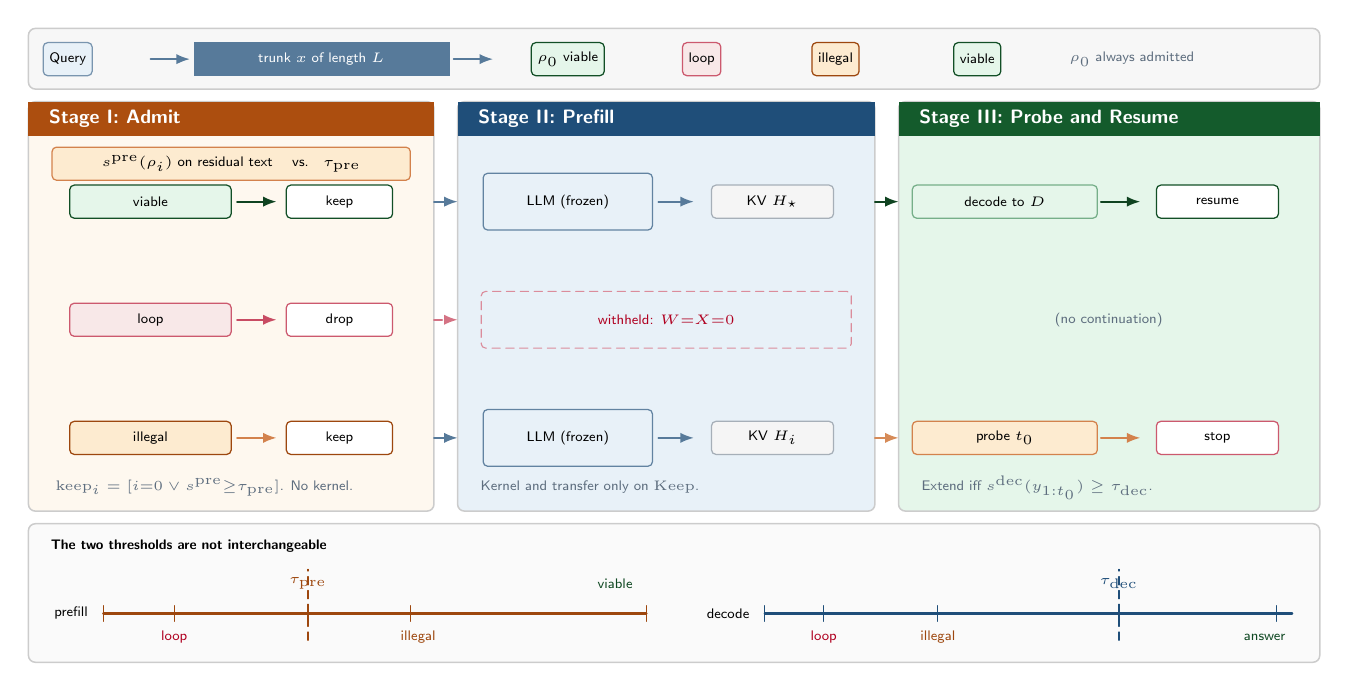
\begin{tikzpicture}[
  x=1cm, y=1cm,
  font=\sffamily\scriptsize,
  >=Latex,
  line cap=round, line join=round,
  panel/.style={draw=black!20, line width=0.55pt, rounded corners=2.5pt, fill=white},
  head/.style={font=\scriptsize\bfseries\sffamily, text=white, anchor=west},
  box/.style={draw, rounded corners=1.6pt, inner sep=2.2pt, font=\tiny\sffamily,
              line width=0.45pt, align=center, minimum height=0.42cm},
  llm/.style={box, draw=fsblue!70, fill=fslight, minimum width=2.15cm, minimum height=0.72cm},
  kv/.style={box, draw=fsgray!55, fill=black!4, minimum width=1.55cm},
  arr/.style={-{Latex[length=1.7mm,width=1.3mm]}, line width=0.62pt, draw=fsblue!75},
]
\path (0,0) rectangle (16.40,8.05);

% ===== query / fan-out =====
\draw[panel, fill=black!3] (0.00,7.28) rectangle (16.40,8.05);
\node[box, draw=fsblue!60, fill=fslight, anchor=west] at (0.18,7.66) {Query};
\draw[arr] (1.55,7.66) -- (2.05,7.66);
\fill[fsblue!75] (2.10,7.44) rectangle (5.35,7.88);
\node[font=\tiny\sffamily, text=white] at (3.72,7.66) {trunk $x$ of length $L$};
\draw[arr] (5.40,7.66) -- (5.90,7.66);
\node[box, fill=fscommit, draw=fsgreen!65!black] at (6.85,7.66) {$\rho_0$ viable};
\node[box, fill=fsmiss, draw=fsred!65] at (8.55,7.66) {loop};
\node[box, fill=fsspec, draw=fsorange!80!black] at (10.25,7.66) {illegal};
\node[box, fill=fscommit, draw=fsgreen!65!black] at (12.05,7.66) {viable};
\node[font=\tiny\sffamily, text=fsgray, anchor=west] at (13.10,7.66) {$\rho_0$ always admitted};

% ===== three stages =====
\draw[panel, fill=fsspec!35] (0.00,1.92) rectangle (5.15,7.12);
\draw[panel, fill=fslight] (5.45,1.92) rectangle (10.75,7.12);
\draw[panel, fill=fscommit] (11.05,1.92) rectangle (16.40,7.12);
\fill[fsorange!88!black] (0.00,6.68) rectangle (5.15,7.12);
\fill[fsblue] (5.45,6.68) rectangle (10.75,7.12);
\fill[fsgreen!75!black] (11.05,6.68) rectangle (16.40,7.12);
\node[head] at (0.14,6.90) {Stage I: Admit};
\node[head] at (5.59,6.90) {Stage II: Prefill};
\node[head] at (11.19,6.90) {Stage III: Probe and Resume};

% --- lane y: viable 5.85, loop 4.35, illegal 2.85 ---
% Stage I scorer
\node[box, draw=fsorange!75, fill=fsspec, minimum width=4.55cm, anchor=north]
  at (2.575,6.55) {$s^{\mathrm{pre}}(\rho_i)$ on residual text \quad vs.\quad $\tau_{\mathrm{pre}}$};

% viable lane
\node[box, fill=fscommit, draw=fsgreen!65!black, minimum width=2.05cm] at (1.55,5.85) {viable};
\draw[arr, draw=fsgreen!55!black] (2.65,5.85) -- (3.15,5.85);
\node[box, fill=white, draw=fsgreen!65!black, minimum width=1.35cm] at (3.95,5.85) {keep};

% loop lane
\node[box, fill=fsmiss, draw=fsred!65, minimum width=2.05cm] at (1.55,4.35) {loop};
\draw[arr, draw=fsred!70] (2.65,4.35) -- (3.15,4.35);
\node[box, fill=white, draw=fsred!65, minimum width=1.35cm] at (3.95,4.35) {drop};

% illegal lane
\node[box, fill=fsspec, draw=fsorange!80!black, minimum width=2.05cm] at (1.55,2.85) {illegal};
\draw[arr, draw=fsorange!75] (2.65,2.85) -- (3.15,2.85);
\node[box, fill=white, draw=fsorange!80!black, minimum width=1.35cm] at (3.95,2.85) {keep};

\node[font=\tiny\sffamily, text=fsgray, align=left, anchor=west] at (0.22,2.22)
  {$\mathrm{keep}_i=[i{=}0\lor s^{\mathrm{pre}}{\ge}\tau_{\mathrm{pre}}]$. No kernel.};

% arrows I -> II
\draw[arr] (5.15,5.85) -- (5.45,5.85);
\draw[arr, draw=fsred!55, densely dashed] (5.15,4.35) -- (5.45,4.35);
\draw[arr] (5.15,2.85) -- (5.45,2.85);

% Stage II
\node[llm] at (6.85,5.85) {LLM (frozen)};
\draw[arr] (8.00,5.85) -- (8.45,5.85);
\node[kv] at (9.45,5.85) {KV $H_{\star}$};

\node[draw=fsred!45, densely dashed, rounded corners=1.6pt, minimum width=4.70cm,
      minimum height=0.72cm] at (8.10,4.35) {};
\node[font=\tiny\sffamily, text=fsred] at (8.10,4.35) {withheld: $W{=}X{=}0$};

\node[llm] at (6.85,2.85) {LLM (frozen)};
\draw[arr] (8.00,2.85) -- (8.45,2.85);
\node[kv] at (9.45,2.85) {KV $H_{i}$};

\node[font=\tiny\sffamily, text=fsgray, align=left, anchor=west] at (5.62,2.22)
  {Kernel and transfer only on $\mathrm{Keep}$.};

% arrows II -> III
\draw[arr, draw=fsgreen!55!black] (10.75,5.85) -- (11.05,5.85);
\draw[arr, draw=fsorange!70] (10.75,2.85) -- (11.05,2.85);

% Stage III
\node[box, draw=fsgreen!60, fill=fscommit, minimum width=2.35cm] at (12.40,5.85) {decode to $D$};
\draw[arr, draw=fsgreen!55!black] (13.62,5.85) -- (14.12,5.85);
\node[box, draw=fsgreen!65!black, fill=white, minimum width=1.55cm] at (15.10,5.85) {resume};

\node[font=\tiny\sffamily, text=fsgray] at (13.72,4.35) {(no continuation)};

\node[box, draw=fsorange!75, fill=fsspec, minimum width=2.35cm] at (12.40,2.85) {probe $t_0$};
\draw[arr, draw=fsorange!75] (13.62,2.85) -- (14.12,2.85);
\node[box, draw=fsred!65, fill=white, minimum width=1.55cm] at (15.10,2.85) {stop};

\node[font=\tiny\sffamily, text=fsgray, align=left, anchor=west] at (11.22,2.22)
  {Extend iff $s^{\mathrm{dec}}(y_{1:t_0})\ge\tau_{\mathrm{dec}}$.};

% ===== number lines =====
\draw[panel, fill=black!2] (0.00,0.00) rectangle (16.40,1.76);
\node[font=\tiny\sffamily\bfseries, anchor=west] at (0.16,1.48)
  {The two thresholds are not interchangeable};

\draw[fsorange!80!black, line width=0.75pt] (0.95,0.62) -- (7.85,0.62);
\node[font=\tiny\sffamily, anchor=east] at (0.88,0.62) {prefill};
\foreach \x in {0.95, 1.85, 3.55, 4.85, 7.85} {
  \draw[fsorange!80!black] (\x,0.52) -- (\x,0.72);
}
\node[font=\tiny\sffamily, text=fsred] at (1.85,0.32) {loop};
\node[font=\tiny\sffamily, text=fsorange!80!black] at (3.55,1.00) {$\tau_{\mathrm{pre}}$};
\node[font=\tiny\sffamily, text=fsorange!80!black] at (4.95,0.32) {illegal};
\node[font=\tiny\sffamily, text=fsgreen!60!black] at (7.45,1.00) {viable};
\draw[fsorange!80!black, densely dashed] (3.55,0.28) -- (3.55,1.18);

\draw[fsblue, line width=0.75pt] (9.35,0.62) -- (16.05,0.62);
\node[font=\tiny\sffamily, anchor=east] at (9.28,0.62) {decode};
\foreach \x in {9.35, 10.10, 11.55, 13.85, 15.85} {
  \draw[fsblue] (\x,0.52) -- (\x,0.72);
}
\node[font=\tiny\sffamily, text=fsred] at (10.10,0.32) {loop};
\node[font=\tiny\sffamily, text=fsorange!80!black] at (11.55,0.32) {illegal};
\node[font=\tiny\sffamily, text=fsblue] at (13.85,1.00) {$\tau_{\mathrm{dec}}$};
\node[font=\tiny\sffamily, text=fsgreen!60!black] at (15.70,0.32) {answer};
\draw[fsblue, densely dashed] (13.85,0.28) -- (13.85,1.18);
\end{tikzpicture}
}
\caption{Illustration of the workflow of \sys.
Given a fan-out with live strategies, a loop, and illegal text, prefill scoring is computed from residual text before any kernel.
A residual is pruned by withholding it from the context KV cache (orange).
Activations after admission are generated only on the admitted cache.
Continuation uses a separate score on a generated prefix of length $t_0$ (green).
The number lines show why the two bars are not interchangeable: illegal text sits above $\tau_{\mathrm{pre}}$ and a still-illegal prefix sits below $\tau_{\mathrm{dec}}$.}
\label{fig:arch}
\end{figure*}

\subsubsection{Prefill Admission}
\label{sec:prefill-admit}

As mentioned in Section~\ref{sec:intro}, we aim at identifying residuals whose text biases the stack toward encoding the same span as a thought rather than as skippable text.
These residuals should not interfere with the model's ability to follow live strategies, i.e., by generating accurate answers that leverage the trunk as supporting context.
The identified residuals are excluded from the KV cache through the following steps.

\paragraph{Scoring.}
Suppose there exists a prefill score $s^{\mathrm{pre}}: \rho \mapsto [0,1]$ that captures the stack's preference over which residuals to encode, i.e., by measuring how much a residual looks like a live strategy rather than a loop.
Residuals scoring below $\tau_{\mathrm{pre}}$ can be viewed as steering the kernel toward wasted prefill.
We score only the residual span $\rho_i$, not the trunk $x$, because abortable text is proposed in the residual.
Details of $s^{\mathrm{pre}}$ are in Section~\ref{sec:scores}.

\paragraph{Forced keep.}
Index $0$ is the residual the search will keep if nothing else survives.
Pruning it would degrade the spine even when every sibling is abortable.
We therefore admit
\begin{equation}
\label{eq:keep}
\mathrm{keep}_i = [\, i = 0 \ \lor\  s^{\mathrm{pre}}(\rho_i) \ge \tau_{\mathrm{pre}} \,].
\end{equation}
Only residuals with $\mathrm{keep}_i$ are queued for the kernel.
$W$ is the measured prefill of that set.
With prefix caching on, a shared trunk is not the dominant term; the gate's effect is that a dropped residual contributes nothing.
The connector inserts KV only for the admitted set, so a dropped residual contributes $X_i = 0$ as well.

\paragraph{Thresholding.}
Pruning residuals with small $s^{\mathrm{pre}}$ should alter the stack's tendency to encode abortable text.
However, this would degrade live answers if $s^{\mathrm{pre}}$ were reused as a decode bar, because that score does not observe a generated prefix.
To maintain quality after pruning, we regularize by a second bar $\tau_{\mathrm{dec}} > \tau_{\mathrm{pre}}$ that is never applied to residual text in the default policy.
Raising the prefill bar to $\tau_{\mathrm{dec}}$ is a faster operating point that we measure, not the default.

\subsubsection{Decode Continuation}
\label{sec:decode-cont}

In experiments, the prefill mask is computed from residual text with no model call, then applied to every fan-out at test time.
Admitted residuals that the decode stage later stops have already paid their prefill; they do not pay the rest of $D$.

Decode length is chosen after admission.
A repeated loop is not probed: it never starts.
Index $0$ and any residual whose planner prior is already at least $\tau_{\mathrm{dec}}$ decode to the budget $D$.
Every other admitted residual decodes $t_0$ tokens, and is extended to $D$ only when a decode score $s^{\mathrm{dec}}$ on the generated prefix clears $\tau_{\mathrm{dec}}$:
\begin{equation}
\label{eq:extend}
\mathrm{extend}_i = [\, s^{\mathrm{dec}}(y_{i,1:t_0}) \ge \tau_{\mathrm{dec}} \,].
\end{equation}
Algorithm~\ref{alg:grow} is this rule.
Section~\ref{sec:hosts} is the special case in which a decode-time host, rather than $t_0$, supplies the later cut.

\begin{algorithm}[t]
\caption{Probe, then extend. Loops skip prefill. Index $0$ decodes to $D$.}
\label{alg:grow}
\begin{algorithmic}[1]
\Require residuals $\rho_{0:k-1}$, budget $D$, probe $t_0$, bars $(\tau_{\mathrm{pre}},\tau_{\mathrm{dec}})$
\For{$i \gets 0$ \textbf{to} $k-1$}
  \If{$i \neq 0$ \textbf{and} $\rho_i$ is a repeated loop}
    \State skip \Comment{no kernel, $X_i{=}0$}
  \ElsIf{$i = 0$ \textbf{or} planner prior of $\rho_i \ge \tau_{\mathrm{dec}}$}
    \State prefill $\rho_i$; decode to $D$
  \Else
    \State prefill $\rho_i$; decode $t_0$ tokens
    \If{$s^{\mathrm{dec}}(y_{i,1:t_0}) \ge \tau_{\mathrm{dec}}$}
      \State extend from $t_0$ to $D$
    \EndIf
  \EndIf
\EndFor
\end{algorithmic}
\end{algorithm}

Applying this mask over the residual ensures that the stack's implicit criteria align with the live--abortable separation already present in the text.
Varying the prefill bar, as in Section~\ref{sec:eval}, shows a trade-off between robustness of any-finished accuracy and quality of following only the winner.

\subsection{The Two Scores}
\label{sec:scores}

As described in Section~\ref{sec:refuse}, admission is guided by $s^{\mathrm{pre}}$ and continuation by $s^{\mathrm{dec}}$.
Both are deterministic functions of a string.
They do not call the model.
They do not share weights.

The prefill scorer looks only at $\rho_i$.
A repeated span is a loop and falls below $\tau_{\mathrm{pre}}$.
A residual that matches an illegal-math pattern, such as a run of stars or an undefined token, lands strictly between $\tau_{\mathrm{pre}}$ and $\tau_{\mathrm{dec}}$.
Any other non-empty residual receives
\begin{equation}
\label{eq:prefill-score}
s^{\mathrm{pre}}(\rho_i) = 0.55\,\min(1, 2\alpha_i) + 0.45\,\min(1, 8\eta_i),
\end{equation}
where $\alpha_i$ is the alphanumeric fraction and $\eta_i$ is the character-level uniqueness.
Live strategy text clears both bars.

The decode scorer looks only at a generated prefix $y_i$.
A repeated prefix stays below $\tau_{\mathrm{dec}}$.
An answer mark (\texttt{\#\#\#\#} or \texttt{\textbackslash boxed}) clears $\tau_{\mathrm{dec}}$.
Illegal text on a prefix also stays below $\tau_{\mathrm{dec}}$, which is why it cannot share $\tau_{\mathrm{pre}}$.
Otherwise
\begin{equation}
\label{eq:decode-score}
\begin{aligned}
s^{\mathrm{dec}}(y_i) = {} & 0.50\,\min(1, 2\alpha) + 0.30\,\min(1, 8\eta) \\
& + 0.20\,\min(1, 20\delta + 15\omega),
\end{aligned}
\end{equation}
with $\delta$ the digit fraction and $\omega$ the fraction of arithmetic symbols.
A static planner prior used by the host-side ranker is a third mix again ($0.35$ alphanumeric, $0.65$ uniqueness) and is never reused as the prefill score.

The operating point is the ordered pair $(\tau_{\mathrm{pre}}, \tau_{\mathrm{dec}})$ with $\tau_{\mathrm{pre}} < \tau_{\mathrm{dec}}$ (Equation~\ref{eq:pair} in the appendix gives the run).
On the prefill axis the loop is below $\tau_{\mathrm{pre}}$ and illegal text is above it, so the gate drops loops and keeps illegal text.
On the decode axis illegal text is below $\tau_{\mathrm{dec}}$ and an answer mark is above it, so a probe stops on illegal text and continues once an answer mark appears.
Section~\ref{sec:eval} measures what happens when a single bar is used for both decisions.

\paragraph{The subset that must survive.}
In Section~\ref{sec:prefill-admit}, we regularize admission by forcing index $0$ and by not using $\tau_{\mathrm{dec}}$ as the default prefill bar.
We want to avoid pruning residuals whose prefill score is that of live strategy text, so that the pruned stack can still generate answers that address the user query by leveraging the trunk.
Index $0$ is among the live set in our evaluation mix, so the forced keep does not add a further slot beyond the live half.
A batch-limited rule that ignores the score and keeps a single residual is a different policy; Section~\ref{sec:eval} shows that it discards correct branches.

\begin{proposition}[Host-invariant prefill]
\label{prop:invariance}
Let $\mathrm{Keep} = \{ i : \mathrm{keep}_i \}$ be the admitted set of \eqref{eq:keep}.
For any decode-time host that scores only generated tokens, the prefill work $W$ equals the measured prefill of $\mathrm{Keep}$ and does not depend on the host.
\end{proposition}
The proof is in Appendix~\ref{app:invariance}.
Proposition~\ref{prop:invariance} is the reason three otherwise different hosts share one prefill column in Figure~\ref{fig:problem}(b) and in Table~\ref{tab:hosts}.

\subsection{The Score Gap}
\label{sec:gap}

Prefill scoring with \eqref{eq:prefill-score} relies on the residual string alone.
Not every abortable residual is a loop.
Specifically, we find that the same illegal span can be interpreted as a thought to encode or as a prefix to stop, depending on whether the score is read before or after generation.
We refer to this phenomenon as the \emph{score gap}.

To illustrate, illegal text scores above $\tau_{\mathrm{pre}}$ on the residual and below $\tau_{\mathrm{dec}}$ on a generated prefix that is still illegal.
A loop is below both bars.
A live residual clears $\tau_{\mathrm{pre}}$; a prefix that has emitted an answer mark clears $\tau_{\mathrm{dec}}$.
Figure~\ref{fig:arch} plots these four points on two number lines.
The gap is why a single bar is the wrong cut: applying $\tau_{\mathrm{dec}}$ as a prefill bar drops illegal residuals that can still solve once a prefix is visible, and applying $\tau_{\mathrm{pre}}$ as a decode bar would extend an illegal prefix that the decode rule is designed to stop.

Motivated by the gap, we perform continuation using only a short prefix of length $t_0$, which has been enough to capture the difference between an illegal prefix and an answer-bearing one.
Compared with decoding every admitted residual to $D$, the probe improves fidelity, since spending the full budget on an illegal prefix introduces additional decode work if a few tokens already suffice to govern the decision.
In experiments, $t_0{=}128$ is the setting that returns MATH-500 any-finished accuracy at $k{=}16$ to the full fan-out.
We do not assume testing prompts contain an answer mark at the first token.

\subsection{In Front of a Decode-Time Host}
\label{sec:hosts}

ESC, speculative rejection, and DPTS remain the decode policy.
\sys only changes the set of residuals that reach them.
\begin{itemize}
  \item ESC decodes an admitted residual out to $D$ while its agreement window is open.
    On this mix the window stays open, so an admitted residual runs to $D{=}512$ and a residual refused by \eqref{eq:keep} is never decoded.
  \item Speculative rejection scores at horizon $\tau{=}256$ and drops the lower fraction $\alpha{=}0.5$ of the admitted set.
    The memory-limit trigger from that paper does not fire at these widths, so $256$ is the cut.
  \item DPTS generates a mini-step of $100$ tokens and early-stops a child whose confidence is below the decode bar.
\end{itemize}
The prefill bar is not retuned per host.
$(\tau_{\mathrm{pre}}, \tau_{\mathrm{dec}})$ is the same pair on all three.
When the prefill bar is raised to $\tau_{\mathrm{dec}}$, the admitted set is the live half.
Those residuals are not the ones the host would have cut, the decode-side drop count falls to zero, and the three hosts converge to the same decode length.
The host remains complementary to \sys, since our approach does not modify the host's scoring rule.

\section{Related Work}
\label{sec:related}

\paragraph{Agentic inference.}
Tree-of-Thoughts proposes candidate thoughts and then values them~\citep{tot}.
Self-consistency draws multiple chains and votes~\citep{selfconsistency}.
ReAct interleaves reasoning with tools~\citep{react}.
ESC closes the sample early once a window of answers agrees~\citep{esc}.
Speculative rejection spends a partial-reward horizon and then drops the lower quantile~\citep{specrej}.
DPTS grows a tree in mini-steps and stops a child whose confidence is low~\citep{dpts}.
In each case the score is a function of generated tokens, so an earlier threshold inside that family shortens decode and leaves prefill unchanged.
The success of those cuts relies on tokens already being resident, i.e., it happens when the stack fails to skip abortable text but still stops it after a prefix.
\sys reads the residual before those tokens exist and leaves the host's cut in place for the residuals it admits.
The decode score is also not a token-draft acceptance test~\citep{speculative}: speculative decoding checks a draft continuation of the same sequence, whereas the probe checks whether a sibling residual should continue to $D$.

\paragraph{Serving.}
Orca batches at iteration granularity~\citep{orca}.
PagedAttention and automatic prefix caching address KV as blocks and reuse a block after its hash is stored~\citep{vllm}; SGLang's radix cache is the same contract for program-structured calls~\citep{sglang}.
DistServe and Splitwise place prefill and decode on separate instances and ship KV across the cut~\citep{distserve,splitwise}.
Those designs remove recomputation of a prefix that has already been stored, and they isolate time-to-first-token from inter-token latency.
The first fan-out of a new trunk has nothing stored, and the connector has no opinion about a residual the search will abort.
Training-time methods that change the model, and test-time workflows that add extra model calls per response, are orthogonal: they require a larger compute budget than a pair of string scores.
\sys is the admission step in front of that kernel and that transfer.
It is complementary to the existing serving stack, while not modifying the prompt or introducing extra test-time overhead in response processing.
Section~\ref{sec:eval} measures the gates.
It does not propose a new page allocator.

\section{Experiments}
\label{sec:eval}

\subsection{Experiment Setup}
\label{sec:setup}

We evaluate \sys on Qwen3-8B at temperature $0$ with prefix caching and tensor parallelism $1$, on four A100 40GB GPUs.
By default we use the ordered pair in Equation~\ref{eq:pair} and probe length $t_0{=}128$.
We evaluate with GSM8K under three decode-time hosts and with MATH-500 under the probe rule.
We also report peak KV, quality, and offered load on a serving stack whose live occupancy is the committed spine, using six model families.
Please refer to Appendix~\ref{app:details} for host parameters and metric definitions.
Note that \sys is complementary to the hosts, since our approach does not modify their scoring rules or require additional test-time model calls.

\paragraph{GSM8K hosts.}
Sixteen GSM8K problems.
Each problem is a fan-out of $k \in \{4,8,16\}$ residuals and a decode budget $D{=}512$.
Each fan-out is a controlled mix: half the residuals are live strategy instructions, and half alternate a repeated loop with illegal text.
Index $0$ is always a live strategy.
\emph{Any-finished} counts a problem if any admitted branch produces the reference number.
\emph{Winner} counts a problem if the branch selected as the winner does.
Both are reported over $16$.
ESC, speculative rejection, and DPTS are the decode hosts.
The host alone submits every residual.
\sys applies $\tau_{\mathrm{pre}}$ first and leaves the host's cut in place.

\paragraph{MATH-500 probe.}
The first $32$ MATH-500 problems at level $4$ or higher, $k \in \{4,8,16\}$, $D{=}1024$.
Half the residuals are contest strategies and half are loops or illegal text.
The decode bar is $\tau_{\mathrm{dec}}$.
Full fan-out decodes every residual to $D$.
Discard drops every residual below that bar before prefill.
Probe admits those residuals for $t_0$ tokens and extends only when the generated prefix clears $\tau_{\mathrm{dec}}$.

\subsection{Result Analysis}
\label{sec:analysis}

We summarize the results in Table~\ref{tab:hosts} and Figure~\ref{fig:results}.
\sys significantly reduces the prefill shared by three decode-time hosts, while maintaining any-finished accuracy.

\begin{table}[t]
\centering
\small
\setlength{\tabcolsep}{4pt}
\begin{tabular}{@{}lrrrr@{}}
\toprule
$k{=}16$ & Prefill & Host & $+\tau_{\mathrm{pre}}$ & Any \\
\midrule
ESC & $5008 \to 3848$ & 17.05\,s & \textbf{14.13\,s} & $16/16$ \\
SR & $5008 \to 3848$ & 13.14\,s & \textbf{12.47\,s} & $16/16$ \\
DPTS & $5008 \to 3848$ & 11.86\,s & \textbf{11.49\,s} & $16/16$ \\
\bottomrule
\end{tabular}
\caption{Prefill pruning at $\tau_{\mathrm{pre}}$ in front of three hosts.
Any-finished stays $16/16$.
The prefill column is identical across hosts because the gate, not the host cut, changes $W$, as predicted by Proposition~\ref{prop:invariance}.}
\label{tab:hosts}
\end{table}

Specifically, with the prefill gate off, the three hosts share one prefill of $5008$ tokens.
Turning on $\tau_{\mathrm{pre}}$ drops the loops, leaves illegal text, and cuts that prefill to $3848$ on every host.
ESC moves the most, because its baseline decodes the loops out to $D$.
Speculative rejection and DPTS move less, because they were already stopping the loop and illegal half at their own cut.
The gate removes the prefill of the loop, which none of those cuts avoids.
This highlights a deficiency of pruning only after tokens exist: the host can stop an abortable residual, but it cannot unspend $W$.

\begin{figure*}[t]
\centering
\resizebox{\textwidth}{!}{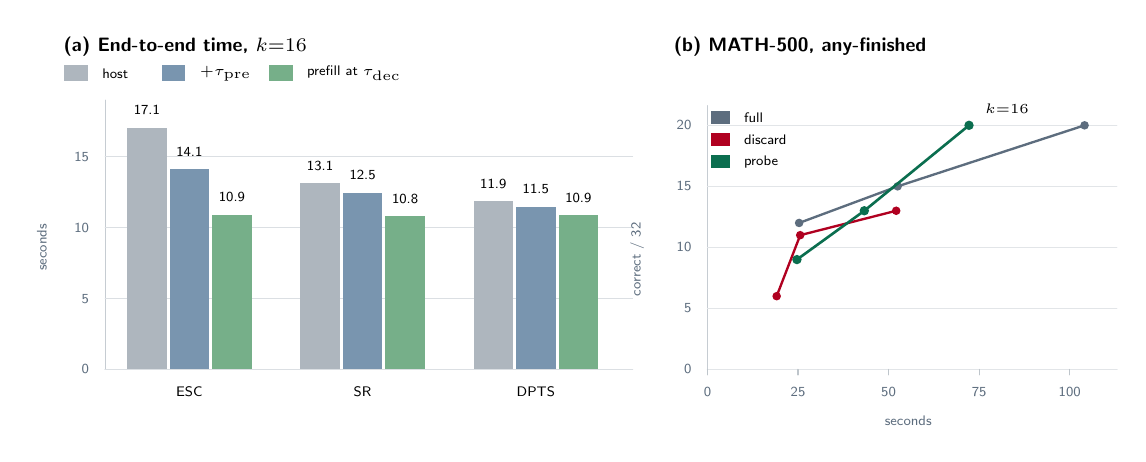
\begin{tikzpicture}[
  x=1cm, y=1cm,
  font=\sffamily\scriptsize,
  >=Latex,
  line cap=round,
]
% ---------- (a) grouped bars, 0.18 cm per second ----------
\node[font=\scriptsize\bfseries\sffamily, anchor=west] at (0.05,4.72) {(a) End-to-end time, $k{=}16$};
\begin{scope}[shift={(0.70,0.62)}]
  \draw[fsgray!35] (0,0) -- (6.70,0);
  \draw[fsgray!35] (0,0) -- (0,3.42);
  \foreach \s/\lab in {0/0, 5/5, 10/10, 15/15} {
    \draw[fsgray!22] (0,{0.18*\s}) -- (6.70,{0.18*\s});
    \node[font=\tiny\sffamily, anchor=east, text=fsgray] at (-0.08,{0.18*\s}) {\lab};
  }
  \node[font=\tiny\sffamily, rotate=90, anchor=south, text=fsgray] at (-0.62,1.55) {seconds};

  \fill[fsgray!50] (0.28,0) rectangle (0.78,{0.18*17.05});
  \fill[fsblue!60] (0.82,0) rectangle (1.32,{0.18*14.13});
  \fill[fsgreen!60] (1.36,0) rectangle (1.86,{0.18*10.92});
  \node[font=\tiny\sffamily, anchor=south] at (0.53,{0.18*17.05+0.04}) {17.1};
  \node[font=\tiny\sffamily, anchor=south] at (1.07,{0.18*14.13+0.04}) {14.1};
  \node[font=\tiny\sffamily, anchor=south] at (1.61,{0.18*10.92+0.04}) {10.9};

  \fill[fsgray!50] (2.48,0) rectangle (2.98,{0.18*13.14});
  \fill[fsblue!60] (3.02,0) rectangle (3.52,{0.18*12.47});
  \fill[fsgreen!60] (3.56,0) rectangle (4.06,{0.18*10.80});
  \node[font=\tiny\sffamily, anchor=south] at (2.73,{0.18*13.14+0.04}) {13.1};
  \node[font=\tiny\sffamily, anchor=south] at (3.27,{0.18*12.47+0.04}) {12.5};
  \node[font=\tiny\sffamily, anchor=south] at (3.81,{0.18*10.80+0.04}) {10.8};

  \fill[fsgray!50] (4.68,0) rectangle (5.18,{0.18*11.86});
  \fill[fsblue!60] (5.22,0) rectangle (5.72,{0.18*11.49});
  \fill[fsgreen!60] (5.76,0) rectangle (6.26,{0.18*10.90});
  \node[font=\tiny\sffamily, anchor=south] at (4.93,{0.18*11.86+0.04}) {11.9};
  \node[font=\tiny\sffamily, anchor=south] at (5.47,{0.18*11.49+0.04}) {11.5};
  \node[font=\tiny\sffamily, anchor=south] at (6.01,{0.18*10.90+0.04}) {10.9};

  \node[font=\tiny\sffamily] at (1.07,-0.28) {ESC};
  \node[font=\tiny\sffamily] at (3.27,-0.28) {SR};
  \node[font=\tiny\sffamily] at (5.47,-0.28) {DPTS};
\end{scope}

\fill[fsgray!50] (0.18,4.28) rectangle (0.48,4.48);
\node[font=\tiny\sffamily, anchor=west] at (0.54,4.38) {host};
\fill[fsblue!60] (1.42,4.28) rectangle (1.72,4.48);
\node[font=\tiny\sffamily, anchor=west] at (1.78,4.38) {$+\tau_{\mathrm{pre}}$};
\fill[fsgreen!60] (2.78,4.28) rectangle (3.08,4.48);
\node[font=\tiny\sffamily, anchor=west] at (3.14,4.38) {prefill at $\tau_{\mathrm{dec}}$};

% ---------- (b) MATH-500 ----------
\begin{scope}[shift={(8.35,0.62)}]
  \node[font=\scriptsize\bfseries\sffamily, anchor=west] at (-0.55,4.10) {(b) MATH-500, any-finished};
  \fill[fsgray] (0.05,3.12) rectangle (0.28,3.28);
  \node[font=\tiny\sffamily, anchor=west] at (0.34,3.20) {full};
  \fill[fsred] (0.05,2.84) rectangle (0.28,3.00);
  \node[font=\tiny\sffamily, anchor=west] at (0.34,2.92) {discard};
  \fill[fsgain] (0.05,2.56) rectangle (0.28,2.72);
  \node[font=\tiny\sffamily, anchor=west] at (0.34,2.64) {probe};

  \draw[fsgray!35] (0,0) -- (5.20,0);
  \draw[fsgray!35] (0,0) -- (0,3.35);
  \foreach \s/\lab in {0/0, 5/5, 10/10, 15/15, 20/20} {
    \draw[fsgray!18] (0,{0.155*\s}) -- (5.20,{0.155*\s});
    \node[font=\tiny\sffamily, anchor=east, text=fsgray] at (-0.08,{0.155*\s}) {\lab};
  }
  \foreach \s/\lab in {0/0, 25/25, 50/50, 75/75, 100/100} {
    \draw[fsgray!40] ({0.046*\s},0) -- ({0.046*\s},-0.07);
    \node[font=\tiny\sffamily, anchor=north, text=fsgray] at ({0.046*\s},-0.10) {\lab};
  }
  \node[font=\tiny\sffamily, text=fsgray, anchor=north] at (2.55,-0.46) {seconds};
  \node[font=\tiny\sffamily, rotate=90, anchor=south, text=fsgray] at (-0.68,1.40) {correct / 32};

  \draw[fsgray, line width=0.85pt] ({0.046*25.3},{0.155*12}) -- ({0.046*52.5},{0.155*15}) -- ({0.046*104.1},{0.155*20});
  \foreach \t/\a in {25.3/12, 52.5/15, 104.1/20} {
    \fill[fsgray] ({0.046*\t},{0.155*\a}) circle (1.55pt);
  }
  \draw[fsred, line width=0.85pt] ({0.046*19.1},{0.155*6}) -- ({0.046*25.6},{0.155*11}) -- ({0.046*52.1},{0.155*13});
  \foreach \t/\a in {19.1/6, 25.6/11, 52.1/13} {
    \fill[fsred] ({0.046*\t},{0.155*\a}) circle (1.55pt);
  }
  \draw[fsgain, line width=0.95pt] ({0.046*24.7},{0.155*9}) -- ({0.046*43.3},{0.155*13}) -- ({0.046*72.2},{0.155*20});
  \foreach \t/\a in {24.7/9, 43.3/13, 72.2/20} {
    \fill[fsgain] ({0.046*\t},{0.155*\a}) circle (1.7pt);
  }
  \node[font=\tiny\sffamily, anchor=south west] at ({0.046*72.2+0.08},{0.155*20+0.02}) {$k{=}16$};
\end{scope}
\end{tikzpicture}
}
\caption{Qwen3-8B.
(a)~GSM8K controlled mix, $k{=}16$, $n{=}16$, $D{=}512$.
Each group is one host.
The gray bar is the host alone, blue adds $\tau_{\mathrm{pre}}$, and green sets the prefill bar to $\tau_{\mathrm{dec}}$.
Any-finished accuracy holds on every bar.
At the higher prefill bar the three hosts meet.
(b)~MATH-500, $n{=}32$, $D{=}1024$.
Each polyline connects $k{=}4$, $k{=}8$, and $k{=}16$.
Discarding residuals below $\tau_{\mathrm{dec}}$ before prefill is fast and less accurate.
The probe under $(\tau_{\mathrm{pre}}, \tau_{\mathrm{dec}})$ meets the full fan-out at $k{=}16$.}
\label{fig:results}
\end{figure*}

Figure~\ref{fig:results}(a) raises the prefill bar from $\tau_{\mathrm{pre}}$ to $\tau_{\mathrm{dec}}$, which also drops illegal text.
Any-finished holds at $k{=}16$.
End-to-end time converges across the three hosts, and the host's later cut fires on nobody: the prefill gate has already removed every residual that cut would have rejected.

\begin{table*}[t]
\centering
\small
\setlength{\tabcolsep}{5pt}
\begin{tabular}{@{}lrrrrrrr@{}}
\toprule
Setting & Admit & Cut later & Prefill & Decode & Time & Any & Winner \\
\midrule
\multicolumn{8}{@{}l}{\emph{Decode pruning only.} No $\tau_{\mathrm{pre}}$. Every residual is prefilled.} \\
ESC, budget $D{=}512$ & 16 & 0 & 5008 & 131072 & 17.05\,s & $16/16$ & $11/16$ \\
SR, horizon $256$ & 16 & 8 & 5008 & 98304 & 13.14\,s & $16/16$ & $12/16$ \\
DPTS, mini-step $100$ & 16 & 8 & 5008 & 78336 & 11.86\,s & $16/16$ & $12/16$ \\
\midrule
\multicolumn{8}{@{}l}{\emph{Prefill pruning only.} Decode runs each admitted residual to $D{=}512$.} \\
$\tau_{\mathrm{pre}}$ & 12 & 0 & 3848 & 98304 & 14.13\,s & $16/16$ & $11/16$ \\
$\tau_{\mathrm{dec}}$ as prefill & 8 & 0 & 2768 & 65536 & \textbf{10.92\,s} & $16/16$ & $10/16$ \\
\midrule
\multicolumn{8}{@{}l}{\emph{Both.} The same prefill bar, then the host cut on what remains.} \\
SR $+\tau_{\mathrm{pre}}$ & 12 & 4 & 3848 & 81920 & 12.47\,s & $16/16$ & $10/16$ \\
DPTS $+\tau_{\mathrm{pre}}$ & 12 & 4 & 3848 & 71936 & 11.49\,s & $16/16$ & $12/16$ \\
SR $+\tau_{\mathrm{dec}}$ & 8 & 0 & 2768 & 65536 & \textbf{10.80\,s} & $16/16$ & $10/16$ \\
DPTS $+\tau_{\mathrm{dec}}$ & 8 & 0 & 2768 & 65536 & \textbf{10.90\,s} & $16/16$ & $10/16$ \\
\bottomrule
\end{tabular}
\caption{Ablation at $k{=}16$ on the GSM8K controlled mix.
``Cut later'' is the number of admitted residuals the host stops at its own horizon.
Any-finished is unchanged.
Winner accuracy moves by at most two problems.
When the prefill bar is $\tau_{\mathrm{dec}}$, the host cut fires on nobody and the decode columns meet.}
\label{tab:ablation}
\end{table*}

Table~\ref{tab:ablation} separates the two gates.
Decode pruning alone never changes prefill, and the time ranking is the ranking of the cut.
Prefill pruning alone, with no host cut, is already faster than ESC at $\tau_{\mathrm{pre}}$ and faster than all three hosts when the prefill bar is $\tau_{\mathrm{dec}}$.
Stacking a host on $\tau_{\mathrm{pre}}$ still stops some of the admitted residuals.
Stacking a host on $\tau_{\mathrm{dec}}$ does not, because the admitted set is the live half.
Any-finished holds throughout.
Winner accuracy is not identical to any-finished: dropping illegal residuals can change which branch the host ranks first.
The gate preserves a correct branch in the admitted set.
Appendix~\ref{app:width} reports $k{=}4$ and $k{=}8$, where the higher prefill bar does drop any-finished accuracy.

The two scores of a loop or an illegal residual are not interchangeable, which is the empirical content of the score gap in Section~\ref{sec:gap}.
On the residual, illegal text lies above $\tau_{\mathrm{pre}}$.
On a generated prefix that is still illegal, the decode score lies below $\tau_{\mathrm{dec}}$.
Applying $\tau_{\mathrm{dec}}$ as a prefill bar therefore drops illegal text, which \eqref{eq:keep} at $\tau_{\mathrm{pre}}$ would have admitted.
On MATH-500 at large $k$ that is the discard row of Table~\ref{tab:probe}.
Applying $\tau_{\mathrm{pre}}$ as a decode bar would do the opposite: an illegal prefix still clears $\tau_{\mathrm{pre}}$, so the probe would extend a residual the decode rule is designed to stop.

\begin{table}[t]
\centering
\small
\setlength{\tabcolsep}{3.5pt}
\begin{tabular}{@{}lccc@{}}
\toprule
 & $k{=}4$ & $k{=}8$ & $k{=}16$ \\
\midrule
Full & 12/32, 25.3\,s & 15/32, 52.5\,s & 20/32, 104.1\,s \\
Discard & 6/32, 19.1\,s & 11/32, 25.6\,s & 13/32, 52.1\,s \\
Probe & 9/32, 24.7\,s & 13/32, 43.3\,s & \textbf{20/32, 72.2\,s} \\
\bottomrule
\end{tabular}
\caption{MATH-500, Qwen3-8B, $n{=}32$, $D{=}1024$.
Each cell is any-finished accuracy and end-to-end time.
At $k{=}16$ the probe matches the full fan-out and is $31\%$ faster.
At $k{=}4$ and $k{=}8$ it does not fully recover accuracy.}
\label{tab:probe}
\end{table}

Table~\ref{tab:probe} and Figure~\ref{fig:results}(b) compare the three prefill policies on MATH-500.
Discarding every residual below $\tau_{\mathrm{dec}}$ is the fastest curve and the least accurate.
The probe spends $t_0$ tokens on the uncertain residuals, then extends a residual only when its prefix clears $\tau_{\mathrm{dec}}$.
At $k{=}16$ any-finished returns to the full fan-out.
At $k{=}4$ and $k{=}8$ it does not.
Recovery is a wide-fan-out result.
Appendix~\ref{app:probe} sweeps $t_0 \in \{64,128\}$, loop-skipping, and a decode-only short budget.
The $k{=}16$ match to full accuracy is specific to $t_0{=}128$ among the probe lengths we compare; $t_0{=}64$ reaches $18/32$.

The prefill gate does not lengthen the committed spine.
Appendix~\ref{app:spine} measures that spine against recomputation and automatic prefix caching.
Peak KV stays below the cache on six model families, because live occupancy is the spine.
On Qwen3-8B the pruned system keeps GSM8K quality with that cache and lowers end-to-end time.
Under a $1$\,s P99 time-to-first-token line, the shorter spine admits a higher offered load.

\begin{table}[t]
\centering
\small
\setlength{\tabcolsep}{4pt}
\begin{tabular}{@{}lrrrr@{}}
\toprule
$k{=}16$, bar $\tau_{\mathrm{dec}}$ & Admit & Prefill & ESC & SR \\
\midrule
Keep one, ignore score & 1 & 414 & $11/16$ & $9/16$ \\
Keep all above $\tau_{\mathrm{dec}}$ & 8 & 2768 & $\mathbf{16/16}$ & $\mathbf{16/16}$ \\
\bottomrule
\end{tabular}
\caption{Winner-only admission on the GSM8K mix.
A single reserved slot drops any-finished accuracy on both hosts.
Scoring, and keeping the whole live half, restores $16/16$.}
\label{tab:best}
\end{table}

Table~\ref{tab:best} holds the batch width fixed and compares two admission rules at $\tau_{\mathrm{dec}}$.
Ignoring the score and keeping one residual drops any-finished accuracy on both hosts.
Keeping every residual at or above $\tau_{\mathrm{dec}}$ restores it.
The savings in Table~\ref{tab:hosts} come from dropping loops, and at $\tau_{\mathrm{dec}}$ from dropping illegal text as well.
They do not come from collapsing the fan-out onto its winner.

\FloatBarrier
\section{Discussion}
\label{sec:discussion}

We presented a lightweight approach to efficient agentic inference.
By identifying and pruning abortable residuals during KV-cache encoding of the residual, and by continuing an uncertain residual only when a short prefix clears a second bar, our approach ensures that prefill and transfer are spent on live strategies rather than on text the search will abort.
Experiments show that \sys exhibits a host-invariant reduction in shared prefill, significantly lowering end-to-end time while preserving large-fan-out any-finished accuracy on GSM8K and MATH-500.
Collapsing either decision onto the other bar, or onto a single reserved slot, is what loses problems.
Our work highlights a practical split for enhancing the efficiency of LLMs in agentic serving, complementary to decode-time hosts, prefix caches, and prefill--decode disaggregation.

\section{Limitations}
\label{sec:limit}

The scores are surface tests: repetition, an illegal-math pattern, an answer mark, and character statistics.
They are not a learned reward model, and a residual that is wrong without being repetitive passes the prefill gate.
The evaluation mix is constructed so that half the fan-out is live strategy text and half is a loop or illegal string.
It is a controlled test of the two thresholds, not a trace of a production agent.
Any-finished accuracy can stay flat while winner accuracy moves, and at $k{=}4$ even $\tau_{\mathrm{pre}}$ drops one GSM8K problem.
The MATH-500 probe recovers full any-finished accuracy at $k{=}16$ and does not do so at $k{=}4$ or $k{=}8$.
The pruning study uses one model and temperature $0$, so the tables are single-run measurements.
The connector numbers in Appendix~\ref{app:xfer} are an accounting model, not a measured transfer time.
We do not explore training-based alternatives such as finetuning a pruner, since we target the setting without a heavy compute budget.


\bibliography{refs}

\appendix

\section{Additional Details}
\label{app:details}

\paragraph{Metrics.}
We evaluate GSM8K with two accuracy numbers and two cost numbers.
Any-finished $\uparrow$ is the fraction of problems for which any admitted residual produces the reference number.
Winner $\uparrow$ is the fraction for which the residual selected as the winner does.
Prefill $\downarrow$ is the measured GPU prefill token total.
Time $\downarrow$ is end-to-end wall-clock seconds on four A100 40GB GPUs.
For MATH-500 we report any-finished and time on the first $32$ problems at level $4$ or higher.
Peak KV is the maximum live bytes of key--value cache; offered load is the concurrent request rate under a $1$\,s P99 time-to-first-token line.

\paragraph{Hosts.}
ESC uses an agreement window of length $5$.
On the controlled mix the window does not fill, so an admitted residual runs to $D{=}512$.
Speculative rejection uses horizon $256$ and dropped fraction $0.5$, applied to the admitted set.
DPTS uses a mini-step of $100$ tokens.
The memory-limit early trigger from speculative rejection does not activate at $k \le 16$ on this hardware.

\paragraph{Admission rules.}
The default rule keeps every residual at or above $\tau_{\mathrm{pre}}$, including index $0$.
Winner-only keeps a single reserved slot and ignores the score.
Both are measured at a fixed batch width in Table~\ref{tab:best}.
\sys is implemented on top of the host-alone baseline.
It is complementary to the hosts, since it does not modify their scoring rules.

\paragraph{Controlled mix.}
For each problem, half of the residuals are live strategy instructions and half alternate a repeated loop with illegal text.
Index $0$ is always live.
The mix is a controlled test of the two bars, not a production trace.
Worked strings are in Appendix~\ref{app:examples}.

\section{Score Functions}
\label{app:scores}

The runs in this paper use one ordered pair,
\begin{equation}
\label{eq:pair}
(\tau_{\mathrm{pre}}, \tau_{\mathrm{dec}}) = (0.15,\ 0.45).
\end{equation}
A loop scores $0.02$ on the residual and $0.04$ on a prefix.
Illegal text scores $0.22$ on the residual and $0.16$ on a prefix.
An answer mark scores $0.92$.
Thus $\tau_{\mathrm{pre}}$ sits between a loop and illegal text, and $\tau_{\mathrm{dec}}$ sits between an illegal prefix and an answer mark.
Raising the prefill bar to $\tau_{\mathrm{dec}}$ is the faster operating point reported in the tables.

Both scorers are deterministic functions of a string.
They do not call the model.
Table~\ref{tab:score-examples} evaluates the residual kinds in the controlled mix.

\begin{table}[h]
\centering
\small
\setlength{\tabcolsep}{4pt}
\begin{tabular}{@{}p{0.42\columnwidth}lcc@{}}
\toprule
Text & Reason & Prefill & Decode \\
\midrule
Repeated \texttt{*loop*} span & loop & 0.02 & 0.04 \\
\texttt{undefined nan \ldots} & illegal & 0.22 & 0.16 \\
Live strategy instruction & ok & $\approx 1.00$ & --- \\
Prefix containing \texttt{\#\#\#\#} or \texttt{\textbackslash boxed} & answer & --- & 0.92 \\
Empty string & empty & 0.00 & 0.00 \\
\bottomrule
\end{tabular}
\caption{Scores on the residual kinds in the evaluation mix.
A dash means that scorer is not applied to that string.
The decode column is the score of a generated prefix of that kind, not a second pass over the residual.}
\label{tab:score-examples}
\end{table}

\paragraph{Prefill.}
After the loop and illegal tests, \eqref{eq:prefill-score} mixes an alphanumeric fraction with character uniqueness.
The coefficients $0.55$ and $0.45$ are fixed.
The measurements score the residual text.

\paragraph{Decode.}
The answer-mark test runs before the illegal test, so a prefix that both looks noisy and contains an answer mark is an answer ($0.92$).
The numeric mix in \eqref{eq:decode-score} adds digit and operator mass so that a healthy math prefix can continue before an answer mark appears.
The planner prior that decides who is probed is
\[
0.35\,\min(1,2\alpha) + 0.65\,\min(1,8\eta)
\]
on the residual, with loop $0.04$ and illegal $0.16$.
It ranks residuals for the host.
It is not substituted for $s^{\mathrm{pre}}$.

\paragraph{Early prefix inside prefill.}
A separate test, not used by the tables in Section~\ref{sec:eval}, inspects the first fraction $\alpha{=}0.20$ of a residual.
It fires when that slice scores below $\tau_{\mathrm{pre}}$ for a reason other than ordinary text.
The reported measurements use the full-residual loop test rather than this partial abort.

\section{Proof of Proposition~\ref{prop:invariance}}
\label{app:invariance}

\begin{proposition*}[Host-invariant prefill]
Let $\mathrm{Keep} = \{ i : \mathrm{keep}_i \}$ be the admitted set of \eqref{eq:keep}.
For any decode-time host that scores only generated tokens, the prefill work $W$ equals the measured prefill of $\mathrm{Keep}$ and does not depend on the host.
\end{proposition*}

\begin{proof}
A decode-time host is a map from generated prefixes to a stop/continue decision~\citep{esc,specrej,dpts}.
By \eqref{eq:decode}, a prefix $y_{i,t}$ exists only after the KV cache $H_i$ of $z_i$ has been encoded.
Therefore the host cannot remove $z_i$ from the prefill batch: its cut acts on decode length, not on whether $\rho_i$ is queued.
Equation~\eqref{eq:keep} is computed from residual text before any kernel, so $\mathrm{Keep}$ is independent of the host.
$W$ is defined as the tokens the kernel runs on that set.
Hence $W$ is a function of $\mathrm{Keep}$ alone.
The three hosts in Table~\ref{tab:hosts} therefore share one prefill column at each bar, and differ only in decode-to-cut.
\end{proof}

The proposition does not claim that end-to-end time is host-invariant.
Time still ranks by the cut: ESC to $D$, speculative rejection to horizon $256$, DPTS to a mini-step of $100$.
Prefill pruning changes the time ranking only by changing $\mathrm{Keep}$, which is the empirical content of Table~\ref{tab:ablation}.

\section{Token Accounting}
\label{app:account}

The decode columns of Table~\ref{tab:ablation} are exact products of the admission counts, the cut, $D{=}512$, and $n{=}16$ problems.
Write $a$ for the number of admitted residuals per problem and $c$ for how many of those the host stops at horizon $h$, with the rest running to $D$.
Decode tokens are $n \bigl(c \cdot h + (a-c) \cdot D\bigr)$.

\begin{itemize}
  \item ESC, no prefill gate: $a{=}16$, $c{=}0$, $h$ unused. $16 \cdot 16 \cdot 512 = 131072$.
  \item Speculative rejection: $a{=}16$, $c{=}8$, $h{=}256$. $16 \cdot (8\cdot 256 + 8\cdot 512) = 98304$.
  \item DPTS: $a{=}16$, $c{=}8$, $h{=}100$. $16 \cdot (8\cdot 100 + 8\cdot 512) = 78336$.
  \item Prefill at $\tau_{\mathrm{pre}}$ only: $a{=}12$, $c{=}0$. $16 \cdot 12 \cdot 512 = 98304$.
  \item Prefill at $\tau_{\mathrm{dec}}$ only: $a{=}8$, $c{=}0$. $16 \cdot 8 \cdot 512 = 65536$.
  \item SR $+\tau_{\mathrm{pre}}$: $a{=}12$, $c{=}4$, $h{=}256$. $16 \cdot (4\cdot 256 + 8\cdot 512) = 81920$.
  \item DPTS $+\tau_{\mathrm{pre}}$: $a{=}12$, $c{=}4$, $h{=}100$. $16 \cdot (4\cdot 100 + 8\cdot 512) = 71936$.
  \item Either host $+\tau_{\mathrm{dec}}$: $a{=}8$, $c{=}0$. $65536$.
\end{itemize}

The mix explains the admission counts.
For $k{=}16$, eight residuals are live and eight are not.
That half alternates loop and illegal text, four of each.
$\tau_{\mathrm{pre}}$ drops the four loops and keeps the four illegal residuals: $8+4=12$.
Raising the prefill bar to $\tau_{\mathrm{dec}}$ drops both kinds: $8$.
Index $0$ is among the live eight, so the forced keep does not add a further slot.
At $k{=}8$ the same halving admits $6$ at $\tau_{\mathrm{pre}}$ and $4$ at $\tau_{\mathrm{dec}}$.
At $k{=}4$ it admits $3$ and $2$.

Prefill tokens are measured, not assigned by this product, because prefix caching makes the incremental prefill depend on the token ids of each residual.
The measured totals at $k{=}16$ are $5008$, $3848$, and $2768$ for admission $16$, $12$, and $8$.
The same totals appear for every host at a given $\tau_{\mathrm{pre}}$, which is the empirical content of Figure~\ref{fig:problem}(b) and of Proposition~\ref{prop:invariance}.

\section{Fan-out Width}
\label{app:width}

\begin{table}[h]
\centering
\small
\setlength{\tabcolsep}{3.2pt}
\resizebox{\columnwidth}{!}{%
\begin{tabular}{@{}lrrrrrr@{}}
\toprule
ESC & Base & $+\tau_{\mathrm{pre}}$ & $\Delta$ & Any & Winner & Prefill \\
\midrule
$k{=}4$ & 8.65\,s & 8.22\,s & $-5\%$ & $16{\to}15$ & $9{\to}9$ & $1320{\to}1018$ \\
$k{=}8$ & 10.84\,s & 10.19\,s & $-6\%$ & $16{\to}16$ & $11{\to}9$ & $2624{\to}2020$ \\
$k{=}16$ & 17.05\,s & 14.13\,s & $-17\%$ & $16{\to}16$ & $11{\to}11$ & $5008{\to}3848$ \\
\bottomrule
\end{tabular}}
\caption{ESC across fan-out width at the default prefill bar.
The relative saving grows with $k$ because more loop residuals are refused.
At $k{=}4$ any-finished drops by one problem.
At $k{=}8$ any-finished holds and the winner moves by two.}
\label{tab:esc-width}
\end{table}

\begin{table}[h]
\centering
\small
\setlength{\tabcolsep}{3.5pt}
\begin{tabular}{@{}lrrrr@{}}
\toprule
 & Prefill & Admit & ESC & Any \\
\midrule
$k{=}16$ base & 5008 & 16 & 17.05\,s & 16/16 \\
$k{=}16$, $\tau_{\mathrm{pre}}$ & 3848 & 12 & 14.13\,s & 16/16 \\
$k{=}16$, $\tau_{\mathrm{dec}}$ as prefill & 2768 & 8 & 10.92\,s & 16/16 \\
$k{=}8$, $\tau_{\mathrm{dec}}$ as prefill & 1448 & 4 & --- & 14/16 \\
$k{=}4$, $\tau_{\mathrm{dec}}$ as prefill & 732 & 2 & --- & 14/16 \\
\bottomrule
\end{tabular}
\caption{Why the default prefill bar is $\tau_{\mathrm{pre}}$.
At $k{=}16$, raising it to $\tau_{\mathrm{dec}}$ is faster and any-finished still holds.
At $k{=}8$ and $k{=}4$ the same bar admits only the live half, which is four and two residuals, and any-finished falls to $14/16$.
Speculative rejection at $k{=}16$ with that higher bar is $10.80$\,s and DPTS is $10.90$\,s, both $16/16$.}
\label{tab:why-015}
\end{table}

The $k{=}4$ row of Table~\ref{tab:esc-width} is the reason Section~\ref{sec:limit} does not describe $\tau_{\mathrm{pre}}$ as accuracy-neutral at every width.
One problem that the full ESC fan-out solved is absent once the single loop residual at $k{=}4$ is refused.
We keep $\tau_{\mathrm{pre}}$ because raising it to $\tau_{\mathrm{dec}}$, which looks better on the $k{=}16$ bars of Figure~\ref{fig:results}(a), fails the same test two widths down (Table~\ref{tab:why-015}).

\section{Probe Sweep}
\label{app:probe}

\begin{table*}[t]
\centering
\small
\setlength{\tabcolsep}{6pt}
\begin{tabular}{@{}lccc@{}}
\toprule
Setting & $k{=}4$ & $k{=}8$ & $k{=}16$ \\
\midrule
Full fan-out & $12/32$, 25.3\,s & $15/32$, 52.5\,s & $20/32$, 104.1\,s \\
Discard every residual below $\tau_{\mathrm{dec}}$ before prefill & $6/32$, 19.1\,s & $11/32$, 25.6\,s & $13/32$, 52.1\,s \\
Drop loops only, decode the rest to $D$ & $11/32$, 23.0\,s & $17/32$, 41.5\,s & $16/32$, 71.4\,s \\
Short-decode the low scores, no extension test & $10/32$, 23.1\,s & $15/32$, 42.3\,s & $17/32$, 74.0\,s \\
Probe $t_0{=}64$, extend iff prefix $\ge \tau_{\mathrm{dec}}$ & $8/32$, 24.0\,s & $16/32$, 42.0\,s & $18/32$, 72.5\,s \\
Probe $t_0{=}128$, extend iff prefix $\ge \tau_{\mathrm{dec}}$ & $9/32$, 24.7\,s & $13/32$, 43.3\,s & $20/32$, 72.2\,s \\
Probe loops as well ($t_0{=}128$) & $10/32$, 24.9\,s & $15/32$, 43.3\,s & $20/32$, 74.4\,s \\
\bottomrule
\end{tabular}
\caption{MATH-500 ablation.
Each cell is any-finished accuracy and wall-clock time.
Dropping loops only is fast and, at $k{=}16$, loses four problems relative to the full fan-out ($16/32$ versus $20/32$).
Probing the non-loop residuals for $128$ tokens and then applying $\tau_{\mathrm{dec}}$ is the only row that matches $20/32$.
Probing the loops too matches accuracy and spends $2.2$\,s more.
At $k{=}8$, several rows land within two problems of the full fan-out; we do not treat a one-problem difference on $n{=}32$ as a ranking.}
\label{tab:probe-full}
\end{table*}

Two comparisons in Table~\ref{tab:probe-full} fix the design of Algorithm~\ref{alg:grow}.
Dropping loops and then decoding everyone else to $D$ is the prefill gate with no probe.
At $k{=}16$ it is slightly faster than the probe ($71.4$\,s versus $72.2$\,s) and four problems less accurate.
The accuracy belongs to the residuals that fail the prefill-side live test and still solve after a prefix is visible.
A short decode that never consults $s^{\mathrm{dec}}$ reaches $17/32$: the extension test, not the mere existence of a short budget, is what returns the last problems.
Including loops in the probe matches $20/32$ at $74.4$\,s.
We still skip loops before the kernel.
Their prefill score is below $\tau_{\mathrm{pre}}$, the probe does not buy accuracy at $k{=}16$, and it spends the extra $2.2$\,s.

At $k{=}16$ and $t_0{=}128$, every non-loop uncertain residual is probed and then extended, and decode tokens fall from $524288$ to $393216$.
The $k{=}8$ probe at $t_0{=}64$ reaches $16/32$, one above the full fan-out's $15/32$.
That is within the one-problem noise we decline to interpret; the claim we use in the body is the $k{=}16$ tie with the full fan-out at lower time.

\section{Host Cuts}
\label{app:hosts}

The three hosts are unchanged except for the set \eqref{eq:keep} hands them.

\paragraph{ESC.}
The published stopping rule waits until a window of agreeing samples is full.
The window length used here is $5$.
The controlled fan-out does not fill that window: some branches are loops or illegal text, and the live strategies do not agree early.
Every admitted residual is therefore decoded to $D$.
This is why ESC's baseline is the most expensive row in Table~\ref{tab:ablation}, and why refusing loops before prefill moves ESC more than it moves DPTS.

\paragraph{Speculative rejection.}
The partial-reward horizon is $\tau{=}256$ tokens and the dropped fraction is $\alpha{=}0.5$, applied to the admitted set rather than to the original $k$.
With $12$ admitted residuals the host stops $4$; with $8$, all eight are above the mass the rule would reject, and the later-cut column is $0$.
The memory-limit early trigger described in that paper does not activate at $k \le 16$ on this hardware, so we do not take credit for it.

\paragraph{DPTS.}
Each admitted child generates a mini-step of $100$ tokens.
A child whose confidence is below $\tau_{\mathrm{dec}}$ stops; the others continue to $D$.
The mini-step is the earliest of the three cuts, which is why DPTS is the fastest host when the prefill gate is off ($11.86$\,s) and why adding the gate moves it by only $0.37$\,s at $\tau_{\mathrm{pre}}$.

\paragraph{Order inside one problem.}
The prefill gate runs before any decode kernel for that fan-out.
The host then runs on the children that were admitted.
Refused residuals are absent from the decode batch.
The gates are ordered by cost: a text test, then prefill, then a short probe or the host horizon, then the rest of $D$.
Only admitted KV is eligible to cross to the decode instance.

\section{Connector Accounting}
\label{app:xfer}

The seconds in Section~\ref{sec:eval} are measured GPU time.
The calculation below is a separate accounting model of the transfer term $X$.

Consider $10$ sessions, $k{=}4$, trunk $L{=}256$, residual length $\ell{=}32$, with one of the four residuals a loop.
A disaggregated prefill that has no admission computes every residual and ships every page:
\[
W = X = 10 \cdot 4 \cdot (256+32) = 11520
\]
tokens.
Charging $12\,\mu\mathrm{s}$ per prefill token and $2\,\mu\mathrm{s}$ per transferred token, plus $0.8$\,ms to abort a refused child, gives a fan-out of $162.1$\,ms of which $23.0$\,ms is transfer.
Refusing the loop before insert leaves three residuals, each still carrying its trunk under this model:
\[
W = X = 10 \cdot 3 \cdot 288 = 8640.
\]
Transfer falls to $17.3$\,ms and the modeled fan-out to $121.8$\,ms.
The $2880$ tokens removed are one residual per session, trunk included, because this model replicates the trunk on the connector.
A page cache that hits the trunk would shrink both the baseline and the pruned column by the same shared prefix; the residual term would remain.
The model shows that the prefill gate and the connector payload move together once admission precedes the transfer.
The measurements already include prefix caching, so the prefill column in Section~\ref{sec:eval} is incremental, not this $11520$-token construction.

\section{Winner-Only Admission}
\label{app:best}

Table~\ref{tab:best} uses batch size $8$ on the $k{=}16$ GSM8K mix at bar $\tau_{\mathrm{dec}}$.
The score-blind rule fills one slot.
Measured prefill is $414$ tokens and any-finished accuracy is $11/16$ under ESC and $9/16$ under speculative rejection.
The score rule admits the eight live residuals ($2768$ prefill tokens) and both hosts return to $16/16$.
The gap is the live strategies other than index $0$.
Several problems are solved by a non-winner live residual and by none of the single reserved slots the blind rule happened to keep.
Keeping the argmax of the prefill score would be a third policy; we do not claim the prefill score ranks answer correctness, only that thresholding it is a different decision from keeping one branch.

\section{Worked Residuals}
\label{app:examples}

The live half cycles through six instructions:

\begin{enumerate}
  \item Translate the story into equations, then solve for the missing value.
  \item Work backwards from the asked quantity to the given numbers.
  \item Name each intermediate quantity in order and add them last.
  \item Build a small table of given facts, then apply one operation at a time.
  \item Estimate the magnitude first, then do exact arithmetic to confirm.
  \item Convert all units, cancel common factors, then compute.
\end{enumerate}

None of them matches the loop or illegal patterns, and \eqref{eq:prefill-score} scores them at $1.0$.
The other half is the alternating pair

\begin{itemize}
  \item a repeated \texttt{*loop*} span, scored $0.02$ because a span of length 8 to 40 repeats at least three extra times;
  \item the string ``undefined nan junk residual that cannot be a proof'', scored $0.22$ by the illegal-math pattern.
\end{itemize}

A generated prefix is scored only after it exists.
The illegal decode score and the answer score in Figure~\ref{fig:arch} are prefix scores.
They are not a second labeling of the residual.

\section{Memory and Offered Load}
\label{app:spine}

\clearpage
The prefill gate does not lengthen the committed spine.
Figures~\ref{fig:eval-multi}, \ref{fig:eval-radar}, and \ref{fig:eval-slo} measure that spine against recomputation and automatic prefix caching on the same serving stack.
Live occupancy is $b(L+\ell_{\star})$ after abort, so peak KV stays below automatic prefix caching.

\begin{figure*}[t]
\centering
\resizebox{\textwidth}{!}{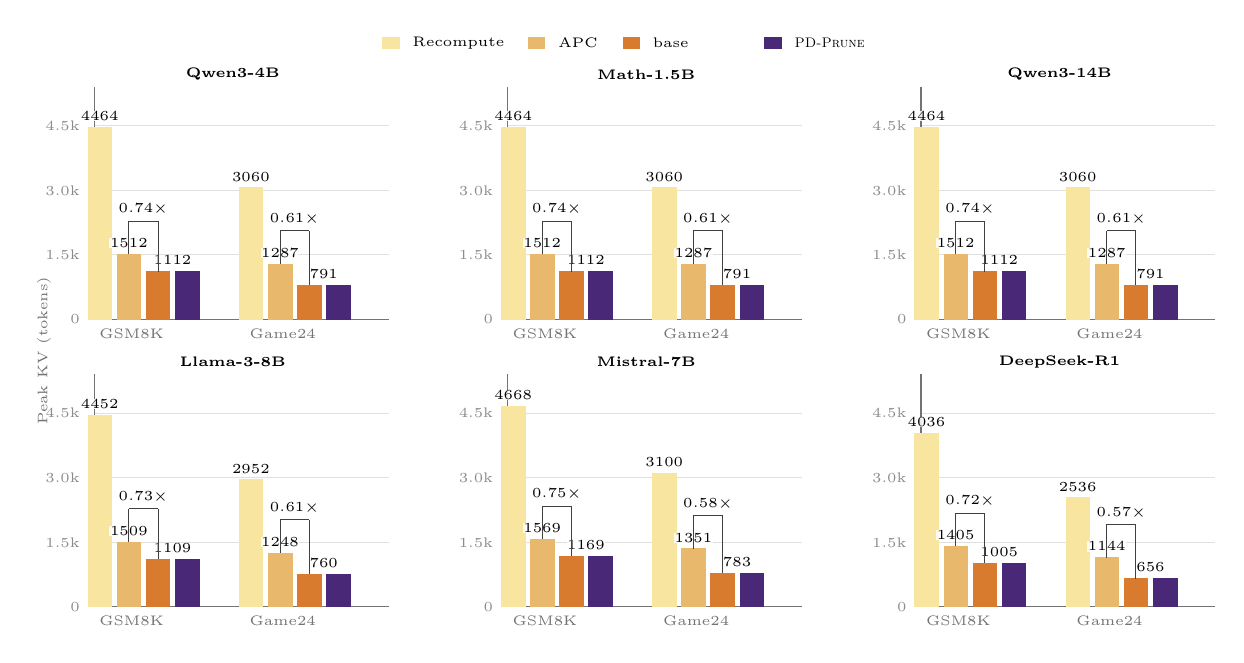
\begin{tikzpicture}[
  font=\scriptsize\sffamily,
  bar/.style={draw=black!65, line width=0.22pt},
  >=Latex,
]
\definecolor{Rec}{HTML}{F8E6A0}
\definecolor{APC}{HTML}{E8B86D}
\definecolor{FS}{HTML}{D97B2F}
\definecolor{FSp}{HTML}{4A2878}

\fill[Rec] (4.10,7.48) rectangle (4.32,7.64);
\node[font=\tiny, anchor=west] at (4.36,7.56) {Recompute};
\fill[APC] (5.95,7.48) rectangle (6.17,7.64);
\node[font=\tiny, anchor=west] at (6.21,7.56) {APC};
\fill[FS] (7.15,7.48) rectangle (7.37,7.64);
\node[font=\tiny, anchor=west] at (7.41,7.56) {base};
\fill[FSp] (8.95,7.48) rectangle (9.17,7.64);
\node[font=\tiny, anchor=west] at (9.21,7.56) {\sys};

% --- Qwen3-4B ---
\begin{scope}[shift={(0.00,3.75)}]
  \node[font=\tiny\bfseries] at (2.20,3.41) {Qwen3-4B};
  \draw[black!12] (0.44,0.300) -- (4.18,0.300);
  \node[font=\tiny, text=black!45, anchor=east] at (0.38,0.300) {0};
  \draw[black!12] (0.44,1.119) -- (4.18,1.119);
  \node[font=\tiny, text=black!45, anchor=east] at (0.38,1.119) {1.5k};
  \draw[black!12] (0.44,1.939) -- (4.18,1.939);
  \node[font=\tiny, text=black!45, anchor=east] at (0.38,1.939) {3.0k};
  \draw[black!12] (0.44,2.758) -- (4.18,2.758);
  \node[font=\tiny, text=black!45, anchor=east] at (0.38,2.758) {4.5k};
  \draw[black!55] (0.44,0.30) -- (4.18,0.30);
  \draw[black!55] (0.44,0.30) -- (0.44,3.25);
  \fill[bar, Rec] (0.360,0.30) rectangle (0.660,2.739);
  \fill[bar, APC] (0.730,0.30) rectangle (1.030,1.126);
  \fill[bar, FS] (1.100,0.30) rectangle (1.400,0.907);
  \fill[bar, FSp] (1.470,0.30) rectangle (1.770,0.907);
  \node[font=\tiny, inner sep=0.2pt, fill=white, fill opacity=0.85, text opacity=1] at (0.510,2.879) {4464};
  \node[font=\tiny, inner sep=0.2pt, fill=white, fill opacity=0.85, text opacity=1] at (0.880,1.266) {1512};
  \node[font=\tiny, inner sep=0.2pt, fill=white, fill opacity=0.85, text opacity=1] at (1.435,1.047) {1112};
  \draw[black!75, line width=0.35pt] (0.880,1.126) -- (0.880,1.546);
  \draw[black!75, line width=0.35pt] (0.880,1.546) -- (1.250,1.546);
  \draw[black!75, line width=0.35pt] (1.250,1.546) -- (1.250,0.907);
  \node[font=\tiny\bfseries] at (1.065,1.696) {$0.74\times$};
  \node[font=\tiny, text=black!55] at (0.915,0.12) {GSM8K};
  \fill[bar, Rec] (2.280,0.30) rectangle (2.580,1.972);
  \fill[bar, APC] (2.650,0.30) rectangle (2.950,1.003);
  \fill[bar, FS] (3.020,0.30) rectangle (3.320,0.732);
  \fill[bar, FSp] (3.390,0.30) rectangle (3.690,0.732);
  \node[font=\tiny, inner sep=0.2pt, fill=white, fill opacity=0.85, text opacity=1] at (2.430,2.112) {3060};
  \node[font=\tiny, inner sep=0.2pt, fill=white, fill opacity=0.85, text opacity=1] at (2.800,1.143) {1287};
  \node[font=\tiny, inner sep=0.2pt, fill=white, fill opacity=0.85, text opacity=1] at (3.355,0.872) {791};
  \draw[black!75, line width=0.35pt] (2.800,1.003) -- (2.800,1.423);
  \draw[black!75, line width=0.35pt] (2.800,1.423) -- (3.170,1.423);
  \draw[black!75, line width=0.35pt] (3.170,1.423) -- (3.170,0.732);
  \node[font=\tiny\bfseries] at (2.985,1.573) {$0.61\times$};
  \node[font=\tiny, text=black!55] at (2.835,0.12) {Game24};
\end{scope}

% --- Math-1.5B ---
\begin{scope}[shift={(5.25,3.75)}]
  \node[font=\tiny\bfseries] at (2.20,3.41) {Math-1.5B};
  \draw[black!12] (0.44,0.300) -- (4.18,0.300);
  \node[font=\tiny, text=black!45, anchor=east] at (0.38,0.300) {0};
  \draw[black!12] (0.44,1.119) -- (4.18,1.119);
  \node[font=\tiny, text=black!45, anchor=east] at (0.38,1.119) {1.5k};
  \draw[black!12] (0.44,1.939) -- (4.18,1.939);
  \node[font=\tiny, text=black!45, anchor=east] at (0.38,1.939) {3.0k};
  \draw[black!12] (0.44,2.758) -- (4.18,2.758);
  \node[font=\tiny, text=black!45, anchor=east] at (0.38,2.758) {4.5k};
  \draw[black!55] (0.44,0.30) -- (4.18,0.30);
  \draw[black!55] (0.44,0.30) -- (0.44,3.25);
  \fill[bar, Rec] (0.360,0.30) rectangle (0.660,2.739);
  \fill[bar, APC] (0.730,0.30) rectangle (1.030,1.126);
  \fill[bar, FS] (1.100,0.30) rectangle (1.400,0.907);
  \fill[bar, FSp] (1.470,0.30) rectangle (1.770,0.907);
  \node[font=\tiny, inner sep=0.2pt, fill=white, fill opacity=0.85, text opacity=1] at (0.510,2.879) {4464};
  \node[font=\tiny, inner sep=0.2pt, fill=white, fill opacity=0.85, text opacity=1] at (0.880,1.266) {1512};
  \node[font=\tiny, inner sep=0.2pt, fill=white, fill opacity=0.85, text opacity=1] at (1.435,1.047) {1112};
  \draw[black!75, line width=0.35pt] (0.880,1.126) -- (0.880,1.546);
  \draw[black!75, line width=0.35pt] (0.880,1.546) -- (1.250,1.546);
  \draw[black!75, line width=0.35pt] (1.250,1.546) -- (1.250,0.907);
  \node[font=\tiny\bfseries] at (1.065,1.696) {$0.74\times$};
  \node[font=\tiny, text=black!55] at (0.915,0.12) {GSM8K};
  \fill[bar, Rec] (2.280,0.30) rectangle (2.580,1.972);
  \fill[bar, APC] (2.650,0.30) rectangle (2.950,1.003);
  \fill[bar, FS] (3.020,0.30) rectangle (3.320,0.732);
  \fill[bar, FSp] (3.390,0.30) rectangle (3.690,0.732);
  \node[font=\tiny, inner sep=0.2pt, fill=white, fill opacity=0.85, text opacity=1] at (2.430,2.112) {3060};
  \node[font=\tiny, inner sep=0.2pt, fill=white, fill opacity=0.85, text opacity=1] at (2.800,1.143) {1287};
  \node[font=\tiny, inner sep=0.2pt, fill=white, fill opacity=0.85, text opacity=1] at (3.355,0.872) {791};
  \draw[black!75, line width=0.35pt] (2.800,1.003) -- (2.800,1.423);
  \draw[black!75, line width=0.35pt] (2.800,1.423) -- (3.170,1.423);
  \draw[black!75, line width=0.35pt] (3.170,1.423) -- (3.170,0.732);
  \node[font=\tiny\bfseries] at (2.985,1.573) {$0.61\times$};
  \node[font=\tiny, text=black!55] at (2.835,0.12) {Game24};
\end{scope}

% --- Qwen3-14B ---
\begin{scope}[shift={(10.50,3.75)}]
  \node[font=\tiny\bfseries] at (2.20,3.41) {Qwen3-14B};
  \draw[black!12] (0.44,0.300) -- (4.18,0.300);
  \node[font=\tiny, text=black!45, anchor=east] at (0.38,0.300) {0};
  \draw[black!12] (0.44,1.119) -- (4.18,1.119);
  \node[font=\tiny, text=black!45, anchor=east] at (0.38,1.119) {1.5k};
  \draw[black!12] (0.44,1.939) -- (4.18,1.939);
  \node[font=\tiny, text=black!45, anchor=east] at (0.38,1.939) {3.0k};
  \draw[black!12] (0.44,2.758) -- (4.18,2.758);
  \node[font=\tiny, text=black!45, anchor=east] at (0.38,2.758) {4.5k};
  \draw[black!55] (0.44,0.30) -- (4.18,0.30);
  \draw[black!55] (0.44,0.30) -- (0.44,3.25);
  \fill[bar, Rec] (0.360,0.30) rectangle (0.660,2.739);
  \fill[bar, APC] (0.730,0.30) rectangle (1.030,1.126);
  \fill[bar, FS] (1.100,0.30) rectangle (1.400,0.907);
  \fill[bar, FSp] (1.470,0.30) rectangle (1.770,0.907);
  \node[font=\tiny, inner sep=0.2pt, fill=white, fill opacity=0.85, text opacity=1] at (0.510,2.879) {4464};
  \node[font=\tiny, inner sep=0.2pt, fill=white, fill opacity=0.85, text opacity=1] at (0.880,1.266) {1512};
  \node[font=\tiny, inner sep=0.2pt, fill=white, fill opacity=0.85, text opacity=1] at (1.435,1.047) {1112};
  \draw[black!75, line width=0.35pt] (0.880,1.126) -- (0.880,1.546);
  \draw[black!75, line width=0.35pt] (0.880,1.546) -- (1.250,1.546);
  \draw[black!75, line width=0.35pt] (1.250,1.546) -- (1.250,0.907);
  \node[font=\tiny\bfseries] at (1.065,1.696) {$0.74\times$};
  \node[font=\tiny, text=black!55] at (0.915,0.12) {GSM8K};
  \fill[bar, Rec] (2.280,0.30) rectangle (2.580,1.972);
  \fill[bar, APC] (2.650,0.30) rectangle (2.950,1.003);
  \fill[bar, FS] (3.020,0.30) rectangle (3.320,0.732);
  \fill[bar, FSp] (3.390,0.30) rectangle (3.690,0.732);
  \node[font=\tiny, inner sep=0.2pt, fill=white, fill opacity=0.85, text opacity=1] at (2.430,2.112) {3060};
  \node[font=\tiny, inner sep=0.2pt, fill=white, fill opacity=0.85, text opacity=1] at (2.800,1.143) {1287};
  \node[font=\tiny, inner sep=0.2pt, fill=white, fill opacity=0.85, text opacity=1] at (3.355,0.872) {791};
  \draw[black!75, line width=0.35pt] (2.800,1.003) -- (2.800,1.423);
  \draw[black!75, line width=0.35pt] (2.800,1.423) -- (3.170,1.423);
  \draw[black!75, line width=0.35pt] (3.170,1.423) -- (3.170,0.732);
  \node[font=\tiny\bfseries] at (2.985,1.573) {$0.61\times$};
  \node[font=\tiny, text=black!55] at (2.835,0.12) {Game24};
\end{scope}

% --- Llama-3-8B ---
\begin{scope}[shift={(0.00,0.10)}]
  \node[font=\tiny\bfseries] at (2.20,3.41) {Llama-3-8B};
  \draw[black!12] (0.44,0.300) -- (4.18,0.300);
  \node[font=\tiny, text=black!45, anchor=east] at (0.38,0.300) {0};
  \draw[black!12] (0.44,1.119) -- (4.18,1.119);
  \node[font=\tiny, text=black!45, anchor=east] at (0.38,1.119) {1.5k};
  \draw[black!12] (0.44,1.939) -- (4.18,1.939);
  \node[font=\tiny, text=black!45, anchor=east] at (0.38,1.939) {3.0k};
  \draw[black!12] (0.44,2.758) -- (4.18,2.758);
  \node[font=\tiny, text=black!45, anchor=east] at (0.38,2.758) {4.5k};
  \draw[black!55] (0.44,0.30) -- (4.18,0.30);
  \draw[black!55] (0.44,0.30) -- (0.44,3.25);
  \fill[bar, Rec] (0.360,0.30) rectangle (0.660,2.732);
  \fill[bar, APC] (0.730,0.30) rectangle (1.030,1.124);
  \fill[bar, FS] (1.100,0.30) rectangle (1.400,0.906);
  \fill[bar, FSp] (1.470,0.30) rectangle (1.770,0.906);
  \node[font=\tiny, inner sep=0.2pt, fill=white, fill opacity=0.85, text opacity=1] at (0.510,2.872) {4452};
  \node[font=\tiny, inner sep=0.2pt, fill=white, fill opacity=0.85, text opacity=1] at (0.880,1.264) {1509};
  \node[font=\tiny, inner sep=0.2pt, fill=white, fill opacity=0.85, text opacity=1] at (1.435,1.046) {1109};
  \draw[black!75, line width=0.35pt] (0.880,1.124) -- (0.880,1.544);
  \draw[black!75, line width=0.35pt] (0.880,1.544) -- (1.250,1.544);
  \draw[black!75, line width=0.35pt] (1.250,1.544) -- (1.250,0.906);
  \node[font=\tiny\bfseries] at (1.065,1.694) {$0.73\times$};
  \node[font=\tiny, text=black!55] at (0.915,0.12) {GSM8K};
  \fill[bar, Rec] (2.280,0.30) rectangle (2.580,1.913);
  \fill[bar, APC] (2.650,0.30) rectangle (2.950,0.982);
  \fill[bar, FS] (3.020,0.30) rectangle (3.320,0.715);
  \fill[bar, FSp] (3.390,0.30) rectangle (3.690,0.715);
  \node[font=\tiny, inner sep=0.2pt, fill=white, fill opacity=0.85, text opacity=1] at (2.430,2.053) {2952};
  \node[font=\tiny, inner sep=0.2pt, fill=white, fill opacity=0.85, text opacity=1] at (2.800,1.122) {1248};
  \node[font=\tiny, inner sep=0.2pt, fill=white, fill opacity=0.85, text opacity=1] at (3.355,0.855) {760};
  \draw[black!75, line width=0.35pt] (2.800,0.982) -- (2.800,1.402);
  \draw[black!75, line width=0.35pt] (2.800,1.402) -- (3.170,1.402);
  \draw[black!75, line width=0.35pt] (3.170,1.402) -- (3.170,0.715);
  \node[font=\tiny\bfseries] at (2.985,1.552) {$0.61\times$};
  \node[font=\tiny, text=black!55] at (2.835,0.12) {Game24};
\end{scope}

% --- Mistral-7B ---
\begin{scope}[shift={(5.25,0.10)}]
  \node[font=\tiny\bfseries] at (2.20,3.41) {Mistral-7B};
  \draw[black!12] (0.44,0.300) -- (4.18,0.300);
  \node[font=\tiny, text=black!45, anchor=east] at (0.38,0.300) {0};
  \draw[black!12] (0.44,1.119) -- (4.18,1.119);
  \node[font=\tiny, text=black!45, anchor=east] at (0.38,1.119) {1.5k};
  \draw[black!12] (0.44,1.939) -- (4.18,1.939);
  \node[font=\tiny, text=black!45, anchor=east] at (0.38,1.939) {3.0k};
  \draw[black!12] (0.44,2.758) -- (4.18,2.758);
  \node[font=\tiny, text=black!45, anchor=east] at (0.38,2.758) {4.5k};
  \draw[black!55] (0.44,0.30) -- (4.18,0.30);
  \draw[black!55] (0.44,0.30) -- (0.44,3.25);
  \fill[bar, Rec] (0.360,0.30) rectangle (0.660,2.850);
  \fill[bar, APC] (0.730,0.30) rectangle (1.030,1.157);
  \fill[bar, FS] (1.100,0.30) rectangle (1.400,0.939);
  \fill[bar, FSp] (1.470,0.30) rectangle (1.770,0.939);
  \node[font=\tiny, inner sep=0.2pt, fill=white, fill opacity=0.85, text opacity=1] at (0.510,2.990) {4668};
  \node[font=\tiny, inner sep=0.2pt, fill=white, fill opacity=0.85, text opacity=1] at (0.880,1.297) {1569};
  \node[font=\tiny, inner sep=0.2pt, fill=white, fill opacity=0.85, text opacity=1] at (1.435,1.079) {1169};
  \draw[black!75, line width=0.35pt] (0.880,1.157) -- (0.880,1.577);
  \draw[black!75, line width=0.35pt] (0.880,1.577) -- (1.250,1.577);
  \draw[black!75, line width=0.35pt] (1.250,1.577) -- (1.250,0.939);
  \node[font=\tiny\bfseries] at (1.065,1.727) {$0.75\times$};
  \node[font=\tiny, text=black!55] at (0.915,0.12) {GSM8K};
  \fill[bar, Rec] (2.280,0.30) rectangle (2.580,1.994);
  \fill[bar, APC] (2.650,0.30) rectangle (2.950,1.038);
  \fill[bar, FS] (3.020,0.30) rectangle (3.320,0.728);
  \fill[bar, FSp] (3.390,0.30) rectangle (3.690,0.728);
  \node[font=\tiny, inner sep=0.2pt, fill=white, fill opacity=0.85, text opacity=1] at (2.430,2.134) {3100};
  \node[font=\tiny, inner sep=0.2pt, fill=white, fill opacity=0.85, text opacity=1] at (2.800,1.178) {1351};
  \node[font=\tiny, inner sep=0.2pt, fill=white, fill opacity=0.85, text opacity=1] at (3.355,0.868) {783};
  \draw[black!75, line width=0.35pt] (2.800,1.038) -- (2.800,1.458);
  \draw[black!75, line width=0.35pt] (2.800,1.458) -- (3.170,1.458);
  \draw[black!75, line width=0.35pt] (3.170,1.458) -- (3.170,0.728);
  \node[font=\tiny\bfseries] at (2.985,1.608) {$0.58\times$};
  \node[font=\tiny, text=black!55] at (2.835,0.12) {Game24};
\end{scope}

% --- DeepSeek-R1 ---
\begin{scope}[shift={(10.50,0.10)}]
  \node[font=\tiny\bfseries] at (2.20,3.41) {DeepSeek-R1};
  \draw[black!12] (0.44,0.300) -- (4.18,0.300);
  \node[font=\tiny, text=black!45, anchor=east] at (0.38,0.300) {0};
  \draw[black!12] (0.44,1.119) -- (4.18,1.119);
  \node[font=\tiny, text=black!45, anchor=east] at (0.38,1.119) {1.5k};
  \draw[black!12] (0.44,1.939) -- (4.18,1.939);
  \node[font=\tiny, text=black!45, anchor=east] at (0.38,1.939) {3.0k};
  \draw[black!12] (0.44,2.758) -- (4.18,2.758);
  \node[font=\tiny, text=black!45, anchor=east] at (0.38,2.758) {4.5k};
  \draw[black!55] (0.44,0.30) -- (4.18,0.30);
  \draw[black!55] (0.44,0.30) -- (0.44,3.25);
  \fill[bar, Rec] (0.360,0.30) rectangle (0.660,2.505);
  \fill[bar, APC] (0.730,0.30) rectangle (1.030,1.068);
  \fill[bar, FS] (1.100,0.30) rectangle (1.400,0.849);
  \fill[bar, FSp] (1.470,0.30) rectangle (1.770,0.849);
  \node[font=\tiny, inner sep=0.2pt, fill=white, fill opacity=0.85, text opacity=1] at (0.510,2.645) {4036};
  \node[font=\tiny, inner sep=0.2pt, fill=white, fill opacity=0.85, text opacity=1] at (0.880,1.208) {1405};
  \node[font=\tiny, inner sep=0.2pt, fill=white, fill opacity=0.85, text opacity=1] at (1.435,0.989) {1005};
  \draw[black!75, line width=0.35pt] (0.880,1.068) -- (0.880,1.488);
  \draw[black!75, line width=0.35pt] (0.880,1.488) -- (1.250,1.488);
  \draw[black!75, line width=0.35pt] (1.250,1.488) -- (1.250,0.849);
  \node[font=\tiny\bfseries] at (1.065,1.638) {$0.72\times$};
  \node[font=\tiny, text=black!55] at (0.915,0.12) {GSM8K};
  \fill[bar, Rec] (2.280,0.30) rectangle (2.580,1.685);
  \fill[bar, APC] (2.650,0.30) rectangle (2.950,0.925);
  \fill[bar, FS] (3.020,0.30) rectangle (3.320,0.658);
  \fill[bar, FSp] (3.390,0.30) rectangle (3.690,0.658);
  \node[font=\tiny, inner sep=0.2pt, fill=white, fill opacity=0.85, text opacity=1] at (2.430,1.825) {2536};
  \node[font=\tiny, inner sep=0.2pt, fill=white, fill opacity=0.85, text opacity=1] at (2.800,1.065) {1144};
  \node[font=\tiny, inner sep=0.2pt, fill=white, fill opacity=0.85, text opacity=1] at (3.355,0.798) {656};
  \draw[black!75, line width=0.35pt] (2.800,0.925) -- (2.800,1.345);
  \draw[black!75, line width=0.35pt] (2.800,1.345) -- (3.170,1.345);
  \draw[black!75, line width=0.35pt] (3.170,1.345) -- (3.170,0.658);
  \node[font=\tiny\bfseries] at (2.985,1.495) {$0.57\times$};
  \node[font=\tiny, text=black!55] at (2.835,0.12) {Game24};
\end{scope}

\node[font=\tiny, text=black!55, rotate=90] at (-0.20,3.65) {Peak KV (tokens)};
\end{tikzpicture}

}
\caption{Peak KV on six models ($n{=}40$, $\mathrm{tp}{=}2$).
Each panel is one family; groups are GSM8K and Game24.
Bars are recompute, APC, the unpruned spine, and \sys.
\sys shares the spine with the unpruned runtime, so the two right-hand bars match.
The annotated ratio is spine over APC.}
\label{fig:eval-multi}
\end{figure*}

\begin{figure*}[t]
\centering
\resizebox{\textwidth}{!}{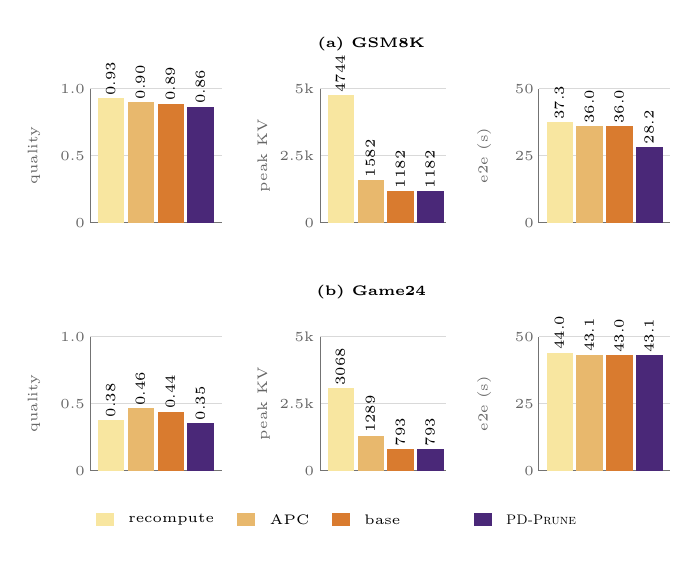
\begin{tikzpicture}[
  font=\scriptsize\sffamily,
  bar/.style={draw=black!55, line width=0.2pt},
  ax/.style={black!55, line width=0.35pt},
  grid/.style={black!15, line width=0.25pt},
  tick/.style={font=\tiny, text=black!60, inner sep=0pt},
  val/.style={font=\tiny, inner sep=0.3pt},
]
\definecolor{Rec}{HTML}{F8E6A0}
\definecolor{APC}{HTML}{E8B86D}
\definecolor{FS}{HTML}{D97B2F}
\definecolor{FSp}{HTML}{4A2878}

% --- (a) GSM8K, y shift 3.15 ---
\begin{scope}[shift={(0,3.15)}]
  \node[font=\tiny\bfseries] at (4.05,2.55) {(a) GSM8K};
  % quality, ymax 1.0
  \begin{scope}[shift={(0,0)}]
    \draw[grid] (0.48,0.28) -- (2.15,0.28) (0.48,1.13) -- (2.15,1.13) (0.48,1.98) -- (2.15,1.98);
    \draw[ax] (0.48,0.28) -- (2.15,0.28) (0.48,0.28) -- (0.48,1.98);
    \node[tick, anchor=east] at (0.42,0.28) {0};
    \node[tick, anchor=east] at (0.42,1.13) {0.5};
    \node[tick, anchor=east] at (0.42,1.98) {1.0};
    \node[tick, rotate=90, anchor=south] at (-0.15,1.13) {quality};
    \fill[bar, Rec] (0.58,0.28) rectangle (0.90,1.853);
    \fill[bar, APC] (0.96,0.28) rectangle (1.28,1.810);
    \fill[bar, FS]  (1.34,0.28) rectangle (1.66,1.788);
    \fill[bar, FSp] (1.72,0.28) rectangle (2.04,1.747);
    \node[val, rotate=90, anchor=west] at (0.74,1.87) {0.93};
    \node[val, rotate=90, anchor=west] at (1.12,1.83) {0.90};
    \node[val, rotate=90, anchor=west] at (1.50,1.81) {0.89};
    \node[val, rotate=90, anchor=west] at (1.88,1.77) {0.86};
  \end{scope}
  % peak KV, ymax 5k
  \begin{scope}[shift={(2.85,0)}]
    \draw[grid] (0.55,0.28) -- (2.15,0.28) (0.55,1.13) -- (2.15,1.13) (0.55,1.98) -- (2.15,1.98);
    \draw[ax] (0.55,0.28) -- (2.15,0.28) (0.55,0.28) -- (0.55,1.98);
    \node[tick, anchor=east] at (0.48,0.28) {0};
    \node[tick, anchor=east] at (0.48,1.13) {2.5k};
    \node[tick, anchor=east] at (0.48,1.98) {5k};
    \node[tick, rotate=90, anchor=south] at (-0.08,1.13) {peak KV};
    \fill[bar, Rec] (0.65,0.28) rectangle (0.97,1.893);
    \fill[bar, APC] (1.03,0.28) rectangle (1.35,0.818);
    \fill[bar, FS]  (1.41,0.28) rectangle (1.73,0.682);
    \fill[bar, FSp] (1.79,0.28) rectangle (2.11,0.682);
    \node[val, rotate=90, anchor=west] at (0.81,1.91) {4744};
    \node[val, rotate=90, anchor=west] at (1.19,0.84) {1582};
    \node[val, rotate=90, anchor=west] at (1.57,0.70) {1182};
    \node[val, rotate=90, anchor=west] at (1.95,0.70) {1182};
  \end{scope}
  % e2e seconds, ymax 50, shorter is faster
  \begin{scope}[shift={(5.70,0)}]
    \draw[grid] (0.48,0.28) -- (2.15,0.28) (0.48,1.13) -- (2.15,1.13) (0.48,1.98) -- (2.15,1.98);
    \draw[ax] (0.48,0.28) -- (2.15,0.28) (0.48,0.28) -- (0.48,1.98);
    \node[tick, anchor=east] at (0.42,0.28) {0};
    \node[tick, anchor=east] at (0.42,1.13) {25};
    \node[tick, anchor=east] at (0.42,1.98) {50};
    \node[tick, rotate=90, anchor=south] at (-0.12,1.13) {e2e (s)};
    \fill[bar, Rec] (0.58,0.28) rectangle (0.90,1.550);
    \fill[bar, APC] (0.96,0.28) rectangle (1.28,1.504);
    \fill[bar, FS]  (1.34,0.28) rectangle (1.66,1.505);
    \fill[bar, FSp] (1.72,0.28) rectangle (2.04,1.239);
    \node[val, rotate=90, anchor=west] at (0.74,1.57) {37.3};
    \node[val, rotate=90, anchor=west] at (1.12,1.52) {36.0};
    \node[val, rotate=90, anchor=west] at (1.50,1.52) {36.0};
    \node[val, rotate=90, anchor=west] at (1.88,1.26) {28.2};
  \end{scope}
\end{scope}

% --- (b) Game24 ---
\begin{scope}[shift={(0,0)}]
  \node[font=\tiny\bfseries] at (4.05,2.55) {(b) Game24};
  \begin{scope}[shift={(0,0)}]
    \draw[grid] (0.48,0.28) -- (2.15,0.28) (0.48,1.13) -- (2.15,1.13) (0.48,1.98) -- (2.15,1.98);
    \draw[ax] (0.48,0.28) -- (2.15,0.28) (0.48,0.28) -- (0.48,1.98);
    \node[tick, anchor=east] at (0.42,0.28) {0};
    \node[tick, anchor=east] at (0.42,1.13) {0.5};
    \node[tick, anchor=east] at (0.42,1.98) {1.0};
    \node[tick, rotate=90, anchor=south] at (-0.15,1.13) {quality};
    \fill[bar, Rec] (0.58,0.28) rectangle (0.90,0.917);
    \fill[bar, APC] (0.96,0.28) rectangle (1.28,1.067);
    \fill[bar, FS]  (1.34,0.28) rectangle (1.66,1.025);
    \fill[bar, FSp] (1.72,0.28) rectangle (2.04,0.875);
    \node[val, rotate=90, anchor=west] at (0.74,0.94) {0.38};
    \node[val, rotate=90, anchor=west] at (1.12,1.09) {0.46};
    \node[val, rotate=90, anchor=west] at (1.50,1.05) {0.44};
    \node[val, rotate=90, anchor=west] at (1.88,0.90) {0.35};
  \end{scope}
  \begin{scope}[shift={(2.85,0)}]
    \draw[grid] (0.55,0.28) -- (2.15,0.28) (0.55,1.13) -- (2.15,1.13) (0.55,1.98) -- (2.15,1.98);
    \draw[ax] (0.55,0.28) -- (2.15,0.28) (0.55,0.28) -- (0.55,1.98);
    \node[tick, anchor=east] at (0.48,0.28) {0};
    \node[tick, anchor=east] at (0.48,1.13) {2.5k};
    \node[tick, anchor=east] at (0.48,1.98) {5k};
    \node[tick, rotate=90, anchor=south] at (-0.08,1.13) {peak KV};
    \fill[bar, Rec] (0.65,0.28) rectangle (0.97,1.323);
    \fill[bar, APC] (1.03,0.28) rectangle (1.35,0.718);
    \fill[bar, FS]  (1.41,0.28) rectangle (1.73,0.550);
    \fill[bar, FSp] (1.79,0.28) rectangle (2.11,0.550);
    \node[val, rotate=90, anchor=west] at (0.81,1.34) {3068};
    \node[val, rotate=90, anchor=west] at (1.19,0.74) {1289};
    \node[val, rotate=90, anchor=west] at (1.57,0.57) {793};
    \node[val, rotate=90, anchor=west] at (1.95,0.57) {793};
  \end{scope}
  \begin{scope}[shift={(5.70,0)}]
    \draw[grid] (0.48,0.28) -- (2.15,0.28) (0.48,1.13) -- (2.15,1.13) (0.48,1.98) -- (2.15,1.98);
    \draw[ax] (0.48,0.28) -- (2.15,0.28) (0.48,0.28) -- (0.48,1.98);
    \node[tick, anchor=east] at (0.42,0.28) {0};
    \node[tick, anchor=east] at (0.42,1.13) {25};
    \node[tick, anchor=east] at (0.42,1.98) {50};
    \node[tick, rotate=90, anchor=south] at (-0.12,1.13) {e2e (s)};
    \fill[bar, Rec] (0.58,0.28) rectangle (0.90,1.775);
    \fill[bar, APC] (0.96,0.28) rectangle (1.28,1.747);
    \fill[bar, FS]  (1.34,0.28) rectangle (1.66,1.741);
    \fill[bar, FSp] (1.72,0.28) rectangle (2.04,1.744);
    \node[val, rotate=90, anchor=west] at (0.74,1.80) {44.0};
    \node[val, rotate=90, anchor=west] at (1.12,1.77) {43.1};
    \node[val, rotate=90, anchor=west] at (1.50,1.76) {43.0};
    \node[val, rotate=90, anchor=west] at (1.88,1.76) {43.1};
  \end{scope}
\end{scope}

\fill[Rec] (0.55,-0.42) rectangle (0.78,-0.26);
\node[font=\tiny, anchor=west] at (0.84,-0.34) {recompute};
\fill[APC] (2.35,-0.42) rectangle (2.58,-0.26);
\node[font=\tiny, anchor=west] at (2.64,-0.34) {APC};
\fill[FS] (3.55,-0.42) rectangle (3.78,-0.26);
\node[font=\tiny, anchor=west] at (3.84,-0.34) {base};
\fill[FSp] (5.35,-0.42) rectangle (5.58,-0.26);
\node[font=\tiny, anchor=west] at (5.64,-0.34) {\sys};
\end{tikzpicture}
}
\caption{Four systems on Qwen3-8B ($n{=}80$, $\mathrm{tp}{=}2$, $D{=}512$).
Each panel has its own axis.
Quality is higher-better; peak KV and end-to-end time are measured values, so a shorter bar is better.
(a)~GSM8K. (b)~Game24.
\sys lowers peak KV below APC on both workloads.
GSM8K quality stays with APC, and \sys also lowers GSM8K end-to-end time.}
\label{fig:eval-radar}
\end{figure*}

\begin{figure}[t]
\centering
\resizebox{\columnwidth}{!}{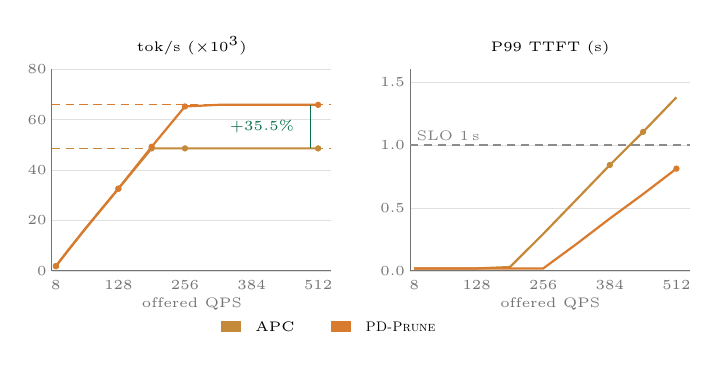
\begin{tikzpicture}[
  font=\scriptsize\sffamily,
  >=Latex,
  tick/.style={font=\tiny, text=black!55, inner sep=0pt},
  grid/.style={black!12, line width=0.25pt},
]
\definecolor{APC}{HTML}{C48A3A}
\definecolor{FSln}{HTML}{D97B2F}

% Measured DeepSeek-R1 GSM8K peaks: APC 761 tok, spine 561 tok.
% 8 GiB pool, 147456 B/token -> C = 76 and 103.
% Service model: e2e = 0.4 s, 256 decode tokens, so one slot is 640 tok/s.
% tok/s = min(round(qps*0.4), C) * 640.
% qps:     8, 32, 64, 128, 192, 256, 320, 384, 448, 512
% APC:  1920, 8320, 16640, 32640, 48640, then 48640
% FS:   1920, 8320, 16640, 32640, 49280, 65280, then 65920
% P99 s, APC: 0.020 until 128, 0.031, 0.294, 0.567, 0.841, 1.104, 1.378
% P99 s, FS:  0.020 until 256, 0.214, 0.416, 0.610, 0.812
% Left y: thousands, 0--80.  x: 512 * 0.0066 = 3.38

\begin{scope}[shift={(0,0)}]
  \foreach \y in {0,20,40,60,80} {
    \draw[grid] (0,\y*0.032) -- (3.55,\y*0.032);
    \node[tick, anchor=east] at (-0.06,\y*0.032) {\y};
  }
  \draw[black!55, line width=0.35pt] (0,0) -- (3.55,0);
  \draw[black!55, line width=0.35pt] (0,0) -- (0,2.56);
  % APC plateau 48.64, spine plateau 65.92
  \draw[APC, densely dashed, line width=0.3pt] (0,48.64*0.032) -- (3.55,48.64*0.032);
  \draw[FSln, densely dashed, line width=0.3pt] (0,65.92*0.032) -- (3.55,65.92*0.032);
  \draw[APC, line width=0.8pt]
    (8*0.0066, 1.92*0.032) -- (32*0.0066, 8.32*0.032) -- (64*0.0066, 16.64*0.032)
    -- (128*0.0066, 32.64*0.032) -- (192*0.0066, 48.64*0.032) -- (512*0.0066, 48.64*0.032);
  \draw[FSln, line width=0.8pt]
    (8*0.0066, 1.92*0.032) -- (32*0.0066, 8.32*0.032) -- (64*0.0066, 16.64*0.032)
    -- (128*0.0066, 32.64*0.032) -- (192*0.0066, 49.28*0.032) -- (256*0.0066, 65.28*0.032)
    -- (320*0.0066, 65.92*0.032) -- (512*0.0066, 65.92*0.032);
  \foreach \q/\ya/\yf in {8/1.92/1.92, 128/32.64/32.64, 192/48.64/49.28, 256/48.64/65.28, 512/48.64/65.92} {
    \fill[APC] (\q*0.0066, \ya*0.032) circle (1.15pt);
    \fill[FSln] (\q*0.0066, \yf*0.032) circle (1.15pt);
  }
  \draw[fsgain, line width=0.4pt] (3.28,48.64*0.032) -- (3.28,65.92*0.032);
  \node[font=\tiny, text=fsgain, anchor=east] at (3.20,1.83) {$+35.5\%$};
  \foreach \q/\lab in {8/8, 128/128, 256/256, 384/384, 512/512} {
    \node[tick] at (\q*0.0066, -0.18) {\lab};
  }
  \node[font=\tiny, anchor=south] at (1.78,2.62) {tok/s ($\times 10^{3}$)};
  \node[tick] at (1.78, -0.42) {offered QPS};
\end{scope}

\begin{scope}[shift={(4.55,0)}]
  \foreach \y in {0.0,0.5,1.0,1.5} {
    \draw[grid] (0,\y*1.60) -- (3.55,\y*1.60);
    \node[tick, anchor=east] at (-0.06,\y*1.60) {\y};
  }
  \draw[black!55, line width=0.35pt] (0,0) -- (3.55,0);
  \draw[black!55, line width=0.35pt] (0,0) -- (0,2.56);
  \draw[black!45, densely dashed] (0,1.60) -- (3.55,1.60);
  \node[tick, anchor=west, text=black!50] at (0.08,1.72) {SLO $1$\,s};
  \draw[APC, line width=0.8pt]
    (8*0.0066, 0.020*1.60) -- (128*0.0066, 0.020*1.60) -- (192*0.0066, 0.031*1.60)
    -- (256*0.0066, 0.294*1.60) -- (320*0.0066, 0.567*1.60) -- (384*0.0066, 0.841*1.60)
    -- (448*0.0066, 1.104*1.60) -- (512*0.0066, 1.378*1.60);
  \draw[FSln, line width=0.8pt]
    (8*0.0066, 0.020*1.60) -- (256*0.0066, 0.020*1.60) -- (320*0.0066, 0.214*1.60)
    -- (384*0.0066, 0.416*1.60) -- (448*0.0066, 0.610*1.60) -- (512*0.0066, 0.812*1.60);
  \fill[APC] (384*0.0066, 0.841*1.60) circle (1.15pt);
  \fill[APC] (448*0.0066, 1.104*1.60) circle (1.15pt);
  \fill[FSln] (512*0.0066, 0.812*1.60) circle (1.15pt);
  \foreach \q/\lab in {8/8, 128/128, 256/256, 384/384, 512/512} {
    \node[tick] at (\q*0.0066, -0.18) {\lab};
  }
  \node[font=\tiny, anchor=south] at (1.78,2.62) {P99 TTFT (s)};
  \node[tick] at (1.78, -0.42) {offered QPS};
\end{scope}

\fill[APC] (2.15,-0.78) rectangle (2.40,-0.64);
\node[font=\tiny, anchor=west] at (2.46,-0.71) {APC};
\fill[FSln] (3.55,-0.78) rectangle (3.80,-0.64);
\node[font=\tiny, anchor=west] at (3.86,-0.71) {\sys};
\end{tikzpicture}
}
\caption{Offered-load sweep from the measured DeepSeek-R1 GSM8K peaks.
Left: saturated tokens per second plateau at concurrency times the decode rate.
Right: APC crosses the $1$\,s P99 line first; \sys stays under it at a higher QPS.}
\label{fig:eval-slo}
\end{figure}



\end{document}
